\documentclass[12pt,aspectratio=169]{beamer}

% ====================================================
% ====================================================
% USEPACKAGES AND IMPORTS
% ====================================================
% ====================================================

\usepackage[T1]{fontenc}
\usepackage[utf8]{inputenc}
\usepackage[english]{babel}

% tables
\usepackage{tabularx}
\usepackage{colortbl}
\usepackage{multirow}
\usepackage{makecell}

% tikz and colors
\usepackage{tikz}
\usepackage{xcolor}
\usepackage{pgfplots}
\usepackage{pgfplotstable}
\usepackage{tikzsymbols}

\usetikzlibrary{calc}
\usetikzlibrary{trees}
\usetikzlibrary{patterns}
\usetikzlibrary{shadings}
\usetikzlibrary{positioning}
\usetikzlibrary{intersections}
\usepgfplotslibrary{patchplots}
\usepgfplotslibrary{fillbetween}
\usetikzlibrary{decorations.pathreplacing}

\usetikzlibrary{arrows}
\usetikzlibrary{arrows.meta}

\usetikzlibrary{shapes}
\usetikzlibrary{shapes.arrows}
\usetikzlibrary{shapes.callouts}
\usetikzlibrary{shapes.symbols}
\usetikzlibrary{shapes.geometric}

% boxes
\usepackage[many]{tcolorbox}

% math packages and fonts
\usepackage{bm}
\usepackage{ccfonts}
\usepackage{eulervm}
\usepackage{amsmath}
\usepackage{amsfonts}
\usepackage{amssymb}
\usepackage{amsthm}
\usepackage{mathtools}
\usepackage{nicefrac}
\usepackage{slashed}
\usepackage{bbold}
\usepackage{array}
\usepackage{cancel}

% algorithms and listings
\usepackage[ruled,vlined,linesnumbered]{algorithm2e}
\usepackage{listings}
\usepackage{setspace}

\tcbuselibrary{listings}
\tcbuselibrary{breakable}
\tcbuselibrary{skins}

% misc
\usepackage{soul}
\usepackage{pifont}
\usepackage{skull}
\usepackage{multicol}
\usepackage{animate}
\usepackage{hyperref}
\usepackage{wasysym}
\usepackage[absolute,overlay]{textpos}
\usepackage[hang,flushmargin]{footmisc}

% ====================================================
% ====================================================
% LAYOUT AND THEME
% ====================================================
% ====================================================

\usetheme{Copenhagen}

% color definitions
\definecolor{myblue1}{RGB}{35,119,189}
\definecolor{myblue2}{RGB}{95,179,238}
\definecolor{myblue3}{RGB}{129,168,207}
\definecolor{myblue4}{RGB}{26,89,142}

\definecolor{myred1}{RGB}{247,12,12}

% set theme colors
\setbeamercolor*{structure}{fg=myblue1,bg=blue}
\setbeamercolor*{palette primary}{use=structure,fg=white,bg=structure.fg}
\setbeamercolor*{palette secondary}{use=structure,fg=white,bg=structure.fg!75!black}
\setbeamercolor*{palette tertiary}{use=structure,fg=white,bg=structure.fg!50!black}
\setbeamercolor*{palette quaternary}{fg=black,bg=white}

\setbeamertemplate{itemize item}[circle]
\setbeamertemplate{itemize subitem}[circle]
\setbeamertemplate{itemize subsubitem}[circle]

\setbeamertemplate{enumerate item}[circle]
\setbeamertemplate{enumerate subitem}[circle]
\setbeamertemplate{enumerate subsubitem}[circle]

\setbeamercolor{itemize item}{fg=myblue1}
\setbeamercolor{itemize subitem}{fg=myblue1}
\setbeamercolor{itemize subsubitem}{fg=myblue1}

\setbeamertemplate{section in toc}[circle]
\setbeamertemplate{subsection in toc}[circle]
\setbeamerfont{subsection in toc}{size=\scriptsize}

\setbeamercolor{frametitle continuation}{fg=black}

% title graphic -- sap logo and dhbw logo
\titlegraphic{
\includegraphics[scale=0.1]{../03_img/logo_sap}\hspace*{4.75cm}~%
   	
\includegraphics[scale=0.05]{../03_img/logo_dhbw}
}

\makeatletter
% frame title
\defbeamertemplate*{frametitle}{mydefault}[1][left]
{
  	\ifbeamercolorempty[bg]{frametitle}{}{\nointerlineskip}%
  	\nointerlineskip%
 	\@tempdima=\textwidth%
  	\advance\@tempdima by\beamer@leftmargin%
  	\advance\@tempdima by\beamer@rightmargin%
  	\begin{tcolorbox}[
  		enhanced,
  		outer arc=0pt,
  		arc=0pt,
  		boxrule=0pt,
  		top=0pt,
  		bottom=0pt,
  		enlarge left by=-\beamer@leftmargin,
  		enlarge right by=-\beamer@rightmargin,
  		width=\paperwidth,
  		nobeforeafter,
  		interior style={
    			left color=myblue2,
    			right color=white
    		},
  		shadow={0mm}{-0.4mm}{0mm}{black!60,opacity=0.6},    
  		shadow={0mm}{-0.8mm}{0mm}{black!40,opacity=0.4},    
  	]
    	\usebeamerfont{frametitle}%
    	\vbox{}\vskip-1ex%
    	\if@tempswa\else\csname beamer@fte#1\endcsname\fi%
    	\insertframetitle\par%
    	{%
      		\ifx\insertframesubtitle\@empty%
      		\else%
      		{\usebeamerfont{framesubtitle}\usebeamercolor[fg]{black}\insertframesubtitle\strut\par}%
      		\fi
    	}%
    	\vskip-1ex%
    	\if@tempswa\else\vskip-.3cm\fi
  	\end{tcolorbox}%
}

% footline of a frame
\defbeamertemplate*{footline}{mysplit theme}
{%
  	\leavevmode%
  	\hbox{
		\begin{beamercolorbox}[
			wd=.5\paperwidth,ht=2.5ex,dp=1.125ex,leftskip=.3cm plus1fill,rightskip=.3cm
		]{author in head/foot}%
    			\usebeamerfont{author in head/foot}\insertshortauthor\ (\insertinstitute), \insertdate
  		\end{beamercolorbox}%
  		\begin{beamercolorbox}[
			wd=.5\paperwidth,ht=2.5ex,dp=1.125ex,leftskip=.3cm,rightskip=.3cm plus1fil
		]{title in head/foot}%
    			\usebeamerfont{title in head/foot}\insertshorttitle\hfill
    			\insertprefix-\insertframenumber/\inserttotalframenumber\hspace*{0.5em}
  		\end{beamercolorbox}}%
  	\vskip0pt%
}
\makeatother

% ====================================================
% ====================================================
% COMMANDS AND GENERAL DEFINITIONS
% ====================================================
% ====================================================

% page number prefix
\newcommand\insertprefix{}  % empty by default
\newcommand\prefix[1]{\renewcommand\insertprefix{#1}}

% math definitions
% ====================================================
\DeclareMathOperator*{\argmax}{arg\,max}
\DeclareMathOperator*{\argmin}{arg\,min}
\newcommand*\diff{\mathop{}\!\mathrm{d}}

\newcommand*{\vertbar}{\rule[-1ex]{0.5pt}{2.5ex}}
\newcommand*{\horzbar}{\rule[.5ex]{2.5ex}{0.5pt}}

% commands
% ====================================================

% highlight commands
% --------------------------------------------------------------------------------------------------------
% highlight command
\newcommand{\highlight}[1]{\textcolor{myblue1}{\textbf{#1}}}
\newcommand{\highlighttt}[1]{\textcolor{myblue1}{\texttt{#1}}}
\newcommand{\Highlight}[1]{\textcolor{myred1}{\textbf{#1}}}

% blue color boxes (with frame/without frame/without fill)
\newtcolorbox{boxBlue}{colback=myblue1!10!white,colframe=myblue4}
\newtcolorbox{boxBlueNoFrame}{colback=myblue1!10!white,colframe=myblue1!10!white}
\newtcolorbox{boxBlueNoFill}{colback=white,colframe=myblue4}

% font commands
% --------------------------------------------------------------------------------------------------------
\newcommand{\linkstyle}[1]{\underline{\smash{\texttt{#1}}}} 		% style of hyperlinks

% tikz commands
% --------------------------------------------------------------------------------------------------------

% yellow sticky note
\newcommand{\bubble}[3]{
\begin{textblock}{100}(#1, #2)
      	\begin{tikzpicture}
		\node[rectangle,draw=yellow,very thick,fill=yellow!60,align=center] at (0,0) {#3};
	\end{tikzpicture}
\end{textblock}
}

\newcommand{\floattext}[3]{
\begin{textblock}{100}(#1, #2)
      	#3
\end{textblock}
}

\newcommand{\doublecircle}[2]{
	\draw[fill=white,draw=myblue1] (#1,#2) circle (2mm);
	\draw[fill=myblue1,draw=myblue1] (#1,#2) circle (1.5mm);
}

% slide modifiers
% --------------------------------------------------------------------------------------------------------
% mark slide as optional
\newcommand{\optional}{
	\begin{textblock}{100}(0.15,0.30)
      		
\includegraphics[scale=0.2]{../03_img/scream}
    	\end{textblock}
}

% mark slide as important
\newcommand{\important}{
	\begin{textblock}{100}(0.10,0.15)
      		
\includegraphics[scale=0.1]{../03_img/important}
    	\end{textblock}
}

% citation
% --------------------------------------------------------------------------------------------------------
% first argument in {book, online, article}
\newcommand{\literature}[5]{
	\setbeamertemplate{bibliography item}[#1]
	\bibitem{#2}
	\highlight{#3} \\
	\textcolor{darkgray}{\textit{#4}} \\
	\textcolor{black}{#5}
}
% cite content
\newcommand{\citeAuthor}[3]{\vfill\scriptsize\textcolor{lightgray}{#1 \cite{#2} #3}}

% slide architecture
% --------------------------------------------------------------------------------------------------------
% divide frame into two parts
\newcommand{\divideTwo}[4]{
	\begin{minipage}{#1\textwidth}
		#2
	\end{minipage}
	\hfill
	\begin{minipage}{#3\textwidth}
		#4
	\end{minipage}
}

% divide frame into two parts (start on top)
\newcommand{\divideTwoTop}[4]{
	\begin{minipage}[t]{#1\textwidth}
		#2
	\end{minipage}
	\hfill
	\begin{minipage}[t]{#3\textwidth}
		#4
	\end{minipage}
}

% special pages
% --------------------------------------------------------------------------------------------------------
% title page
\newcommand{\maketitlepage}{
	{
		\beamertemplatenavigationsymbolsempty
		\usebackgroundtemplate{%
			\tikz[overlay,remember picture] \node[opacity=0.2, at=(current page.center)] {
  				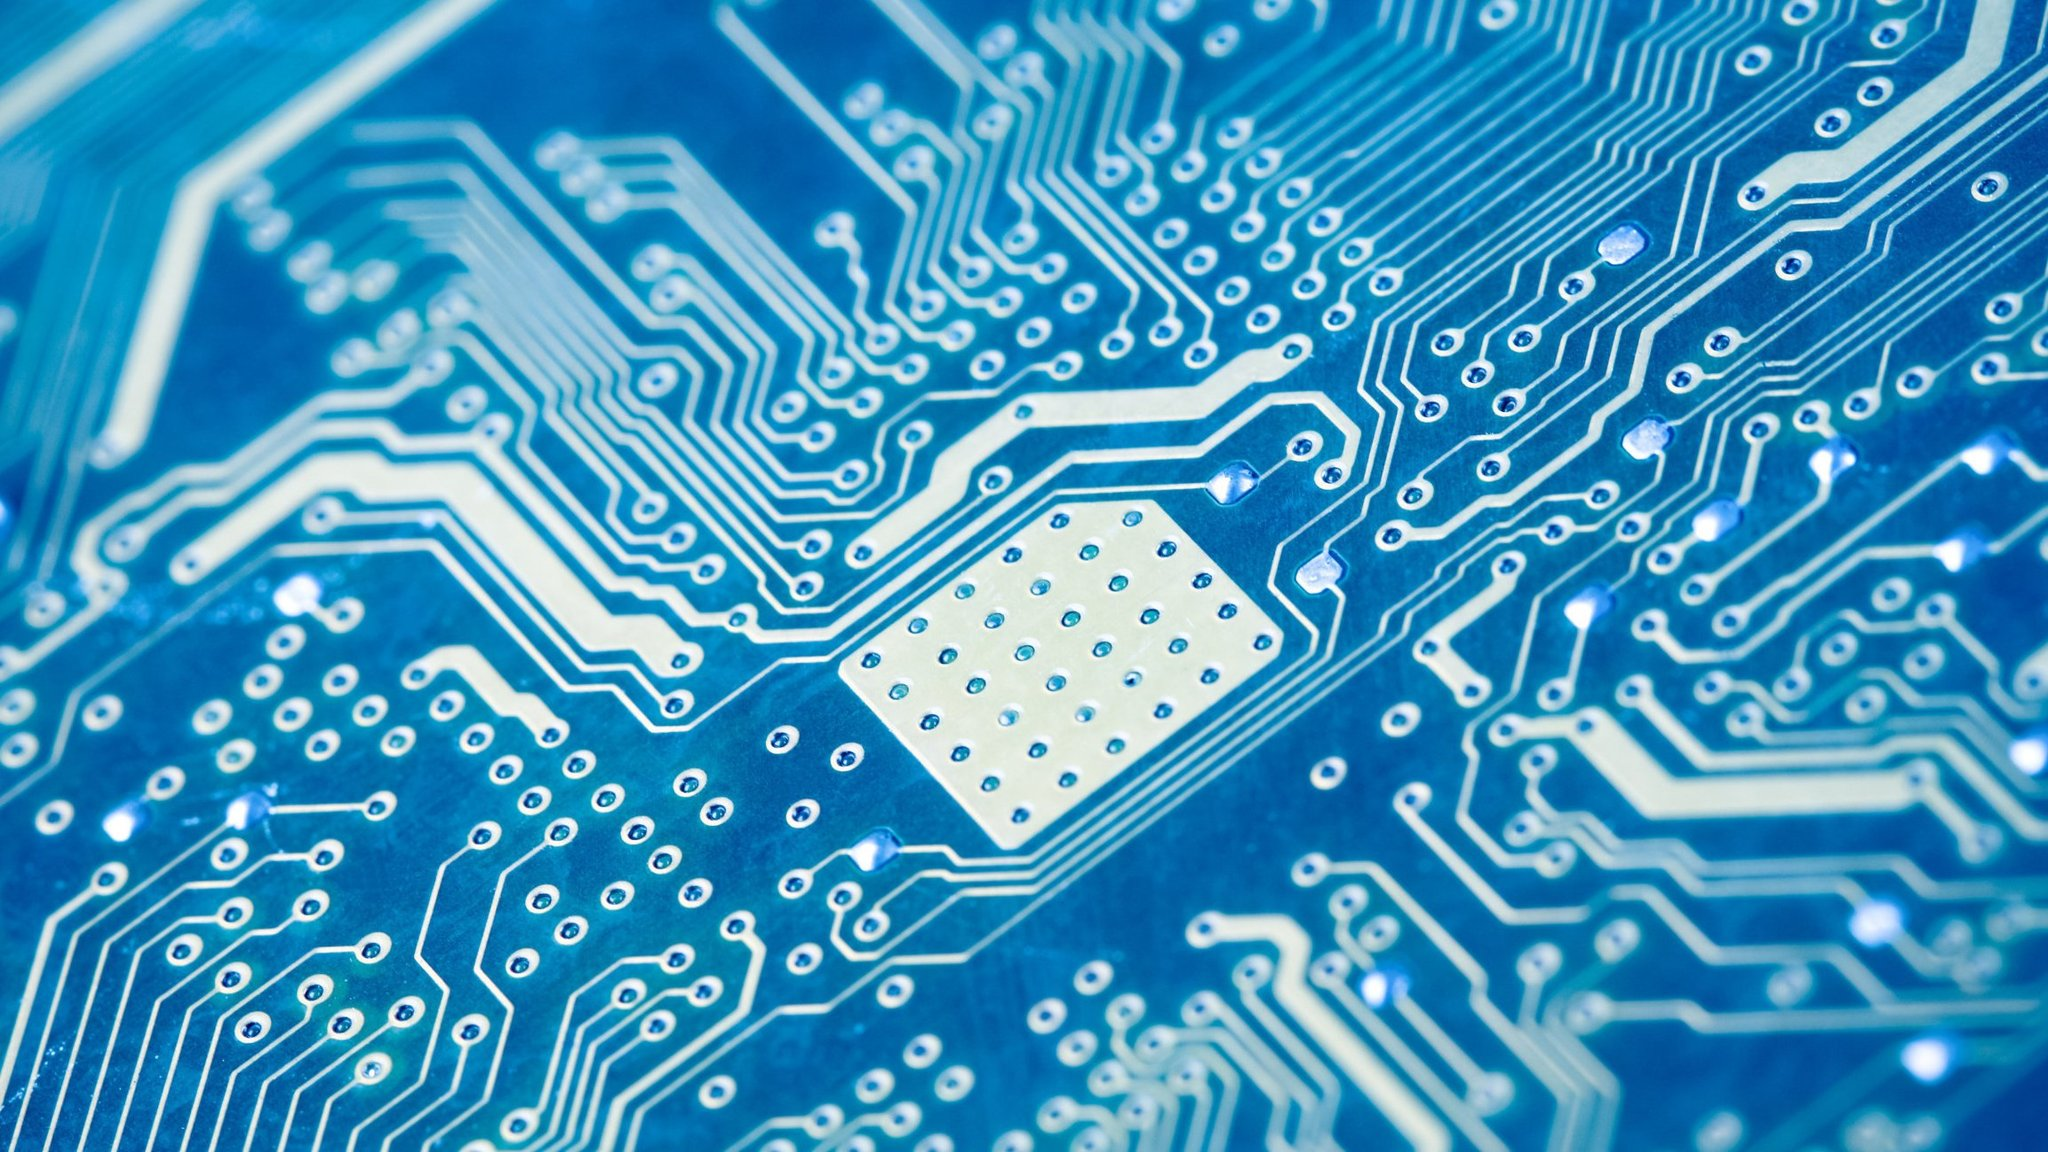
\includegraphics[height=\paperheight,width=\paperwidth]{../03_img/processor.jpg}
			};
		}
		\begin{frame}[plain]
			\vspace*{0.75cm}
			\maketitle
			\vfill
			\begin{center}
				\footnotesize Find all slides on \href{https://github.com/DaWe1992/Applied_ML_Fundamentals}{\linkstyle{GitHub}}
			\end{center}
		\end{frame}
	}
}

% divider page
\newcommand{\makedivider}[1]{
	{
		\beamertemplatenavigationsymbolsempty
		\usebackgroundtemplate{%
			\tikz[overlay,remember picture] \node[opacity=0.2, at=(current page.center)] {
  				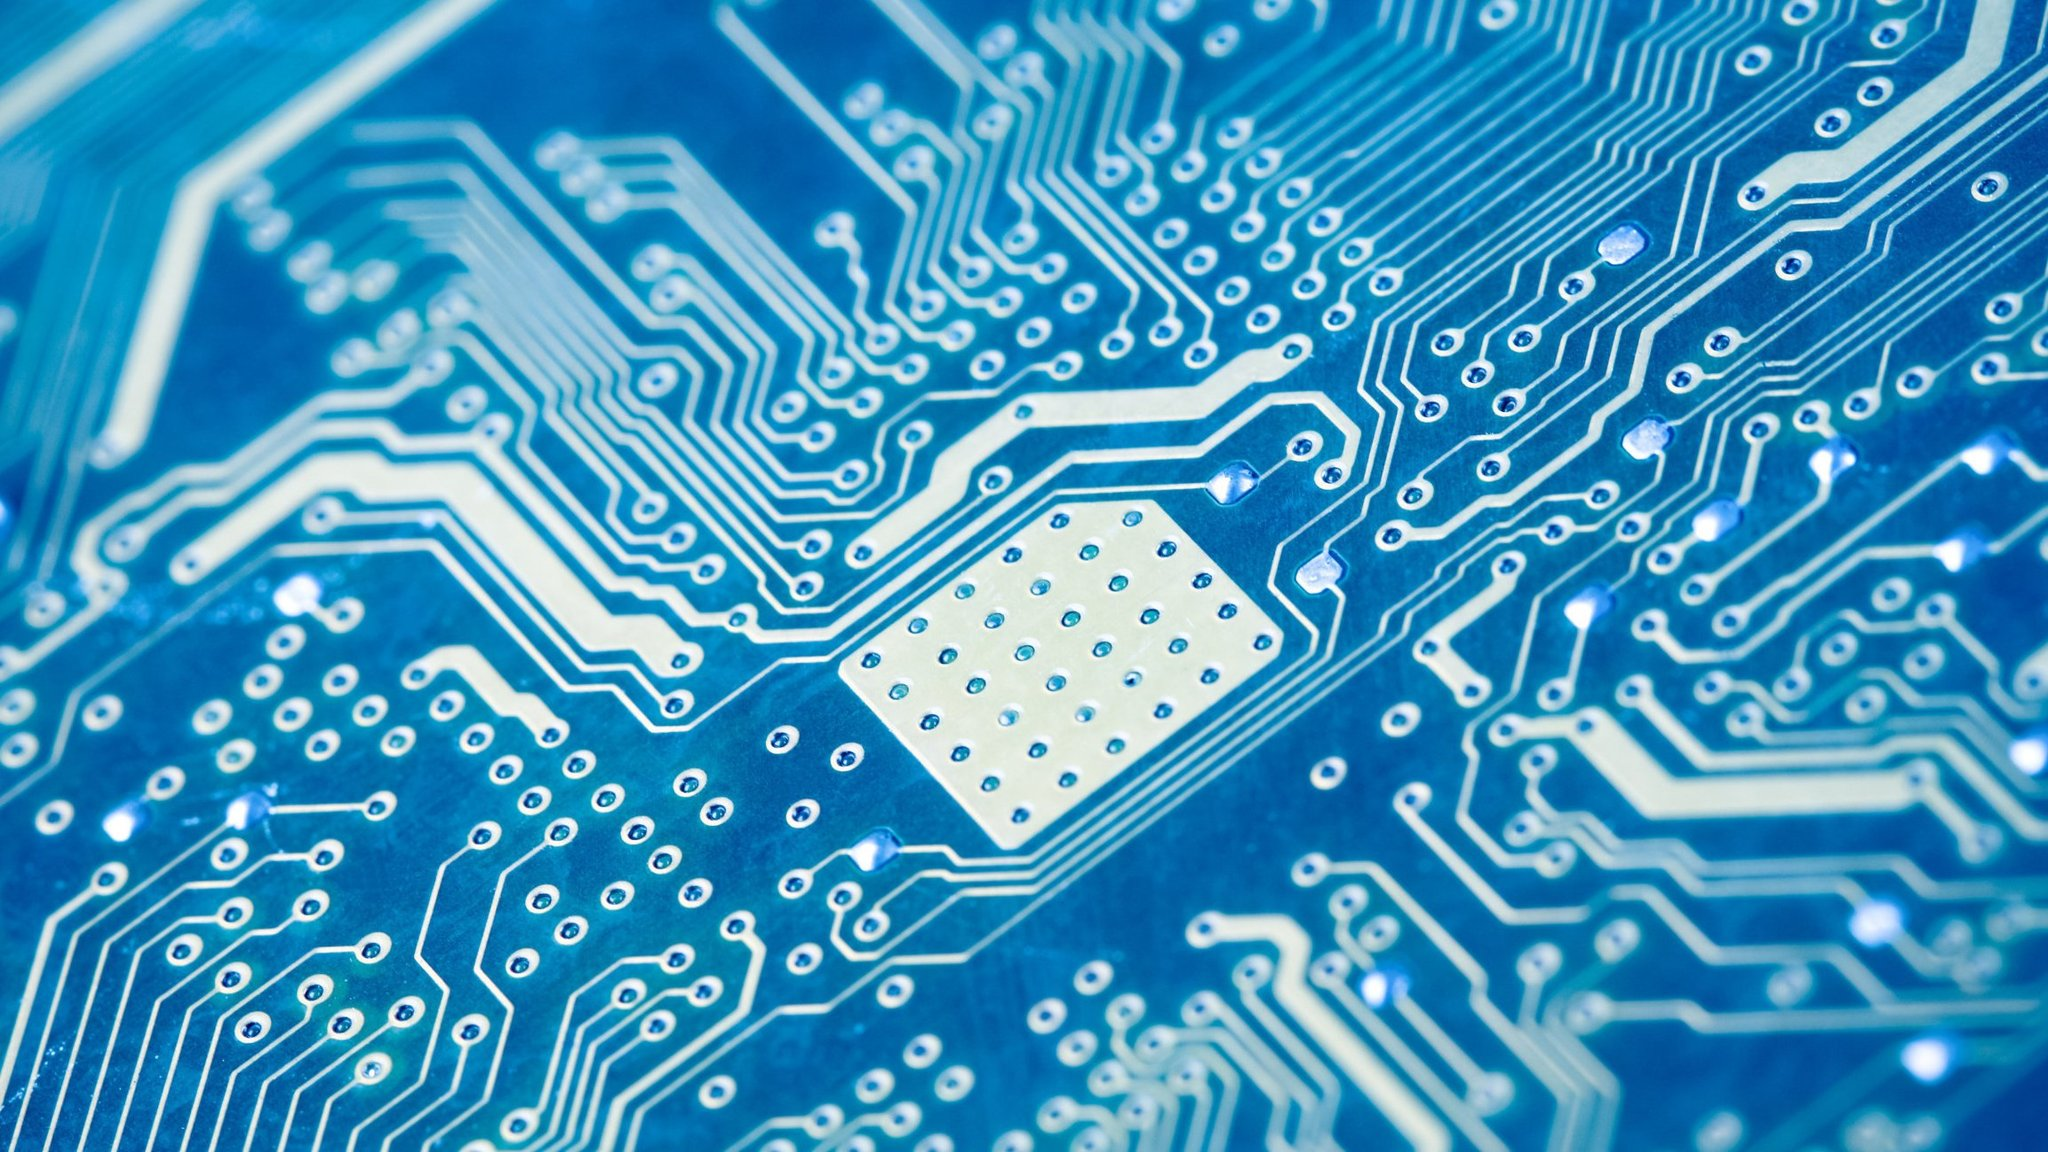
\includegraphics[height=\paperheight,width=\paperwidth]{../03_img/processor.jpg}
			};
		}
		\begin{frame}[plain]
			\vfill
			\begin{boxBlue}
				\centering
				\textbf{Section:} \\
				\large \highlight{#1}
			\end{boxBlue}
			\vfill
			\centering
			
\includegraphics[scale=0.05]{../03_img/logo_dhbw.png}
			\vfill
		\end{frame}
	}
}

% overview page
\newcommand{\makeoverview}[1]{
	\begin{frame}{Lecture Overview}{}
		\begin{tabbing}
			\hspace*{3.5cm}\= \kill
			\ifnum #1=1 \highlight{\textbf{Unit I:}} \else \textbf{Unit I:} \fi
			\> \ifnum #1=1 \highlight{Machine Learning Introduction} \else Machine Learning Introduction \fi \\
		\end{tabbing}
	\end{frame}
}

% thank you page
\newcommand{\makethanks}{
	{\beamertemplatenavigationsymbolsempty
	\begin{frame}[plain]
		\vfill
		\begin{boxBlue}
			\centering
			\Large \highlight{Thank you very much for the attention!}
		\end{boxBlue}
		
		\vfill\footnotesize
		\begin{tabbing}
			\hspace*{1.5cm}\= \kill
			\highlight{Topic:} 	\> \inserttitle \\
			\highlight{Date:} 	\> \insertdate
		\end{tabbing}
		
		\vfill
		\highlight{Contact:} \\
		\insertauthor\ (D062271) \\
		\insertinstitute \\
		\href{mailto:daniel.wehner@sap.com}{\linkstyle{daniel.wehner@sap.com}}
		
		\vfill\normalsize
		\begin{center}
			\large\highlight{Do you have any questions?}
		\end{center}
		\vfill
	\end{frame}}
}

% global pfgplots settings
% --------------------------------------------------------------------------------------------------------
\pgfplotsset{
	% allow filtering of data for pgfplots
	discard if/.style 2 args={
        		x filter/.code={
            		\edef\tempa{\thisrow{#1}}
            		\edef\tempb{#2}
            		\ifx\tempa\tempb
                		\def\pgfmathresult{inf}
            		\fi
        		}
    	},
    	discard if not/.style 2 args={
        		x filter/.code={
            		\edef\tempa{\thisrow{#1}}
            		\edef\tempb{#2}
            		\ifx\tempa\tempb
            		\else
                		\def\pgfmathresult{inf}
            		\fi
        		}
    	}
}

\usepackage{hyperref}

% ====================================================
% ====================================================
% PRESENTATION DATA
% ====================================================
% ====================================================

\title[Mathematical Foundations]{*** Applied Machine Learning Fundamentals *** Mathematical Foundations}
\institute{SAP\,SE}
\author{Daniel Wehner}
\date{\today}
\prefix{MATH}

% ====================================================
% ====================================================
% BEGIN OF DOCUMENT
% ====================================================
% ====================================================

\begin{document}

% Title frame
%______________________________________________________________________
\maketitlepage


% Lecture Overview
%______________________________________________________________________
\begin{frame}{Lecture Overview}{}
	\makeoverview{2}
\end{frame}


% Agenda
%______________________________________________________________________
\begin{frame}{Agenda \today}
	\begin{multicols}{2}
		\tableofcontents
	\end{multicols}
\end{frame}


% Section: Introduction
%______________________________________________________________________
\section{Introduction}
\makedivider{Introduction}

% Introduction
\begin{frame}{Introduction}{}
	\begin{boxBlueNoFrame}
		\highlight{Math is a significant portion of data science / machine learning!}
	\end{boxBlueNoFrame}
	\divideTwo{0.39}{
		\begin{figure}
			\centering
			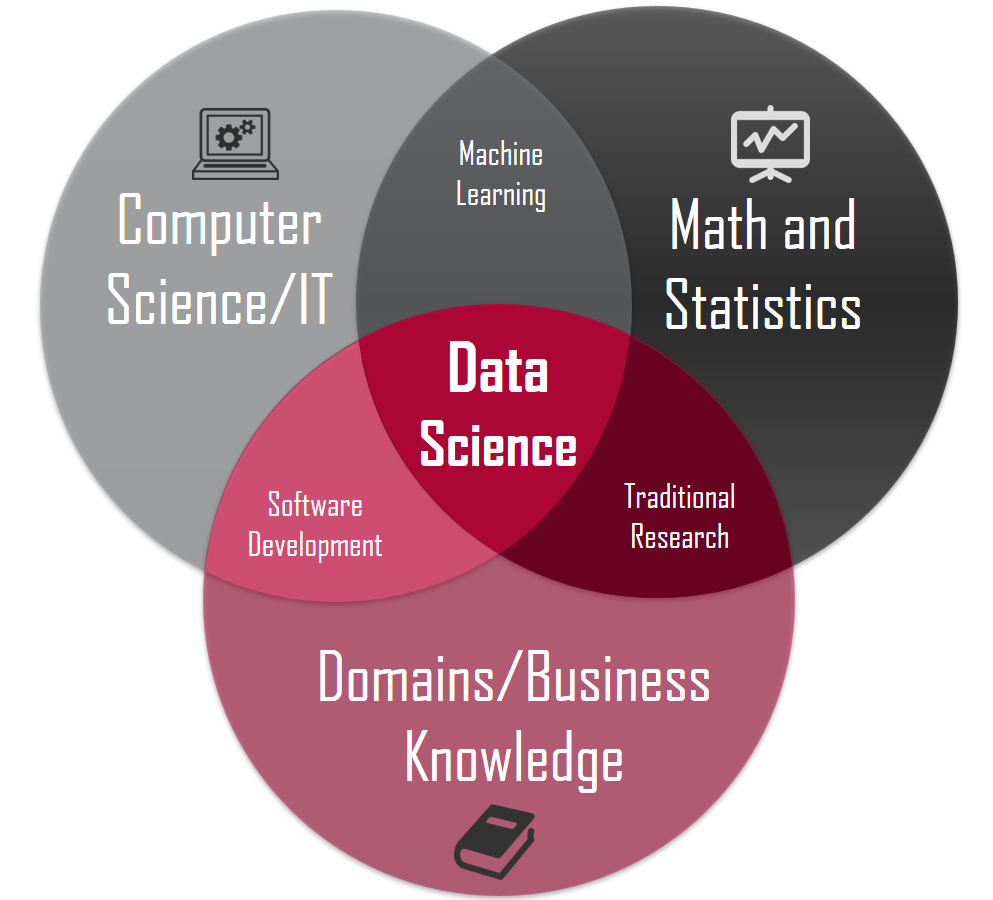
\includegraphics[scale=0.125]{02_math/02_img/data_science.png}
		\end{figure}
	}{0.59}{
		\vspace{0.5cm}
		You will need it to understand:
		\begin{itemize}
			\item \textbf{Statistical} machine learning
			\item How optimization for learning / empirical risk minimization works,
			\item How linear algebra, calculus and statistics are used to make learning and inference more efficient
		\end{itemize}
	}
\end{frame}


% Math is important!
\begin{frame}{Math is important!}{}
	\begin{figure}
	\centering
	\begin{tikzpicture}
		\pie[pos ={0,0}, radius=2, text=legend,explode=0.2]{
			35/Linear algebra,
			25/Probability theory and statistics,
			15/Multivariate calculus,
			15/Algorithms and complexity,
			10/Others
		}
	\end{tikzpicture}
\end{figure}
\end{frame}


% Section: Linear Algebra
%______________________________________________________________________
\section{Linear Algebra}
\makedivider{Linear Algebra}

% Subsection: Vectors
% --------------------------------------------------------------------------------------------------------
\subsection{Vectors}

% What is a Vector?
\begin{frame}{What is a Vector?}{}
	\divideTwo{0.49}{
		\begin{align*}
			\bm{x} 	&= \left[\begin{array}{C{1em}} $x_1$ \\ $x_2$ \end{array}\right] 	\\[4mm]
			\bm{v} 	&= \left[\begin{array}{C{1em}} $3$ \\ $1$ \end{array}\right] 		\\[4mm]
			\bm{w} 	&= \left[\begin{array}{C{1em}} $2$ \\ $4$ \end{array}\right]
		\end{align*}
	}{0.49}{
		\begin{figure}
	\centering
	\begin{tikzpicture}[
		scale=0.8,
		axis/.style={
			->,ultra thick
		}
	]
	
		% draw grid
		\draw[lightgray] (0,0) grid (5,5);
		
		\draw[very thick,myblue1,-stealth] (0,0) -- (3,1) node[right=3mm,fill=myblue1!30] {$\bm{x}^{(1)}$};
		\draw[very thick,gray,-stealth] (0,0) -- (2,4) node[right=3mm,fill=lightgray!50] {$\bm{x}^{(2)}$};
	
		% draw axes
		\draw[axis] (0,0) -- (0,5) node[above]{$x_2$}; \draw[axis] (0,0) -- (5,0) node[right]{$x_1$};
		% axis labels
		\foreach \x in {0,1,...,5} \node at (\x,-0.5){\footnotesize{\x}};
		\foreach \y in {0,1,...,5} \node at (-0.5,\y){\footnotesize{\y}};

	\end{tikzpicture}
\end{figure}
	}
\end{frame}


% Multiplication by a Scalar
\begin{frame}{Multiplication by a Scalar}{}
	\divideTwo{0.49}{
		\begin{align*}
			c \bm{x}
				&= c \left[\begin{array}{C{1em}} $x_1$ \\ $x_2$ \end{array}\right]
					= \left[\begin{array}{C{1em}} $c x_1$ \\ $c x_2$ \end{array}\right]	\\[4mm]
			2 \bm{v} 
				&= 2 \left[\begin{array}{C{1em}} $3$ \\ $1$ \end{array}\right]
					= \left[\begin{array}{C{1em}} $6$ \\ $2$ \end{array}\right]
		\end{align*}
	}{0.49}{
		\begin{figure}
	\centering
	\begin{tikzpicture}[
		scale=0.4
	]

		\draw[very thick,blue,-stealth] (0,0) -- (7,2.8) node[below=1mm] {$c\bm{x}$};
		\draw[ultra thick,red,-stealth] (0,0) -- (5,2) node[below=1mm] {$\bm{x}$};

	\end{tikzpicture}
\end{figure}
	}
\end{frame}


% Addition of Vectors
\begin{frame}{Addition of Vectors}{}
	\divideTwo{0.59}{
		\begin{align*}
			\bm{x} + \bm{y} = \left[\begin{array}{C{1em}} $x_1$ \\ $x_2$ \end{array}\right] +
					\left[\begin{array}{C{1em}} $y_1$ \\ $y_2$ \end{array}\right]
				&= \left[\begin{array}{C{3em}} $x_1 + y_1$ \\ $x_2 + y_2$ \end{array}\right] \\[4mm]
			\bm{v} + \bm{w} = \left[\begin{array}{C{1em}} $3$ \\ $1$ \end{array}\right] +
					\left[\begin{array}{C{1em}} $2$ \\ $4$ \end{array}\right]
				&= \left[\begin{array}{C{1em}} $5$ \\ $5$ \end{array}\right]
		\end{align*}
	}{0.39}{
		\begin{figure}
	\centering
	\begin{tikzpicture}[
		scale=0.5
	]

		\draw[ultra thick,red,-stealth] (0,0) -- (5,2) node[below=1mm] {$\bm{x}$};
		\draw[ultra thick,blue,-stealth] (0,0) -- (1,3) node[left=1mm] {$\bm{y}$};

		\draw[thick,red,dashed] (1,3) -- (6,5);
		\draw[ultra thick,gray,-stealth] (0,0) -- (6,5) node[right] {$\bm{x} + \bm{y}$};

	\end{tikzpicture}
\end{figure}
	}
\end{frame}


% Linear Combination of Vectors
\begin{frame}{Linear Combination of Vectors}{}
	\vspace*{-4mm}
	\begin{align}
		\bm{u} = c_1 \bm{v}^{(1)} + c_2 \bm{v}^{(2)} + \dots + c_n \bm{v}^{(n)}
	\end{align}
	\begin{figure}
	\centering
	\begin{tikzpicture}[
		scale=0.8,
		axis/.style={
			->,ultra thick
		}
	]
	
		% draw grid
		\draw[lightgray] (0,0) grid (6,4);

		\fill[lightgray!30] (0,0) -- (4,4) -- (6,4) -- (6,1.5) -- cycle;
		
		\draw[thick,myblue1!70,-stealth] (0,0) -- (1.5,1.5);
		\draw[thick,lightgray,-stealth] (0,0) -- (3,0.75);

		\draw[very thick,myblue1,-stealth] (0,0) -- node[above=3mm] {\footnotesize $\bm{v}^{(1)}$} (1,1);
		\draw[very thick,gray,-stealth] (0,0) -- (2,0.5) node[below right=-2mm and 0.4mm] {\footnotesize $\bm{v}^{(2)}$};

		\draw[dashed] (1.5,1.5) -- (4.5,2.25);
		\draw[dashed] (3,0.75) -- (4.5,2.25);

		\draw[ultra thick,-stealth] (0,0) -- (4.5,2.25) node[right] {\footnotesize $\bm{u}$};
	
		% draw axes
		\draw[axis] (0,0) -- (0,4) node[above]{$x_2$}; \draw[axis] (0,0) -- (6,0) node[right]{$x_1$};
		% axis labels
		\foreach \x in {0,1,...,6} \node at (\x,-0.5){\footnotesize{\x}};
		\foreach \y in {0,1,...,4} \node at (-0.5,\y){\footnotesize{\y}};

	\end{tikzpicture}
\end{figure}
\end{frame}


% Vector Transpose, inner and outer Product
\begin{frame}{Vector Transpose, inner and outer Product}{}\important
	\begin{itemize}
		\item Vector transpose:
		\begin{equation*}
			\bm{v} = \left[\begin{array}{C{1em}} $3$ \\ $1$ \end{array}\right] \qquad\qquad
			\bm{v}^{\intercal} = \left[\begin{array}{C{1em} C{1em}} $3$ & $1$ \end{array}\right]
		\end{equation*}
		\item Inner product / dot product / scalar product:
		\begin{align}
			\bm{v} \cdot \bm{w}
				&\equiv \bm{v}^{\intercal} \bm{w} \equiv \langle \bm{v}, \bm{w} \rangle
					= \sum_{j=1}^m v_j w_j \\[1mm]
				\nonumber
				&= \left[\begin{array}{C{1em} C{1em}} $3$ & $1$ \end{array}\right]
					\left[\begin{array}{C{1em}} $2$ \\ $4$ \end{array}\right]
					= (3 \cdot 2) + (1 \cdot 4) = 10
		\end{align}
	\end{itemize}
\end{frame}


% Vector Transpose and inner and outer Product (Ctd.)
\begin{frame}{Vector Transpose and inner and outer Product (Ctd.)}{}\important
	\begin{itemize}
		\item Outer product:
		\begin{equation*}
			\bm{v}\bm{w}^{\intercal}
				= 	\left[\begin{array}{C{1em}} $3$ \\ $1$ \end{array}\right]
						\left[\begin{array}{C{1em} C{1em}} $2$ & $4$ \end{array}\right]
				= 	\left[\begin{array}{C{1em} C{1em}} $6$ & $12$ \\ $2$ & $4$ \end{array}\right]
		\end{equation*}
	\end{itemize}

	\begin{boxBlueNoFrame}
		\highlight{The inner product yields a scalar value, the results of an outer product is a matrix!}
	\end{boxBlueNoFrame}
\end{frame}


% Length of a Vector
\begin{frame}{Length of a Vector}{}
	\begin{itemize}
		\item Length of a vector (Frobenius norm):
		\begin{align}
			\Vert \bm{x} \Vert
				&= \sqrt{\bm{x}^{\intercal} \bm{x}}		\\[1mm]
			\Vert c \bm{x} \Vert
				&= \vert c \vert \cdot \Vert \bm{x} \Vert	\\[1mm]
			\Vert \bm{x} + \bm{y} \Vert
				&\le \Vert \bm{x} \Vert + \Vert \bm{y} \Vert
		\end{align}
		\item Example:
		\begin{equation*}
			\Vert \bm{v} \Vert = \sqrt{3^2 + 1^2} = 10
		\end{equation*}
	\end{itemize}
\end{frame}


% Angle between Vectors
\begin{frame}{Angle between Vectors}{}
	\begin{itemize}
		\item The angle between two vectors is given by:
		\begin{align}
			\cos \measuredangle (\bm{x}, \bm{y}) &= \frac{\bm{x} \cdot \bm{y}}{\Vert \bm{x} \Vert \cdot \Vert \bm{y} \Vert}
				= \frac{\sum_{j=1}^m x_j \cdot y_j}{\sqrt{\sum_{j=1}^m (x_j)^2} \cdot \sqrt{\sum_{j=1}^m (y_j)^2}} \\[3mm]
			\nonumber
			\cos \measuredangle (\bm{v}, \bm{w}) &= \frac{\bm{v} \cdot \bm{w}}{\Vert \bm{v} \Vert \cdot \Vert \bm{w} \Vert}
				= \frac{10}{\sqrt{10} \cdot \sqrt{20}} \approx 0.71
		\end{align}
		\vspace*{1mm}
		\item Inner product: $\bm{x} \cdot \bm{y}
			= \Vert \bm{x} \Vert \cdot \Vert \bm{y} \Vert \cdot \cos \measuredangle (\bm{x}, \bm{y})$
	\end{itemize}
\end{frame}


% Projection of Vectors
\begin{frame}{Projection of Vectors}{}
	\floattext{12}{5}{
		\begin{tikzpicture}[
	scale=0.5
]

	\coordinate (A) at ($(0,0)!(3,4)!(5,1)$);
	\draw[dashed,thick] (3,4) -- (A);
		
	\draw[very thick,red,-stealth] (0,0) -- (5,1) node[right] {$\bm{v}$};
	\draw[very thick,blue,-stealth] (0,0) -- (3,4) node[right] {$\bm{w}$};

	\draw[decorate,decoration={brace,amplitude=10pt},xshift=-4pt,yshift=0pt] (A) -- (0,0);
	\node at (2,-1) {$p$};

\end{tikzpicture}

	}
	\begin{itemize}
		\item How is the projection of $\bm{x}$ onto $\bm{y}$ defined?
		\item Formally, we have:
		\begin{align}
			\nonumber
			p 	&= \Vert \bm{v} \Vert \cos \measuredangle (\bm{v}, \bm{w}) 							\\[1mm]
			\nonumber
				&= \Vert \bm{v} \Vert \frac{\bm{v} \cdot \bm{w}}{\Vert \bm{v} \Vert \cdot \Vert \bm{w} \Vert} 	\\[1mm]
				&= \frac{\bm{v} \cdot \bm{w}}{\Vert \bm{w} \Vert}
		\end{align}
		\item Note that $p$ is \textbf{not a vector!}
	\end{itemize}
\end{frame}


% Subsection: Matrices
% --------------------------------------------------------------------------------------------------------
\subsection{Matrices}

% What is a Matrix?
\begin{frame}{What is a Matrix?}{}
	\vspace*{-3mm}
	\divideTwo{0.49}{
		General case ($\mathbb{R}^{n \times m}$):
		\begin{equation*}
			\bm{X}
				= 	\left[\begin{array}{C{1.5em} C{1.5em} C{1.5em} C{1.5em}}
						$X_{11}$ 	& 	$X_{12}$ 	& 	$\hdots$ & 	$X_{1m}$ 	\\
						$X_{21}$ 	& 	$X_{22}$ 	& 	$\hdots$ &	$X_{2m}$ 	\\
						$\vdots$  	& 	$\vdots$		& 	$\ddots$ & 	$\vdots$		\\
						$X_{n1}$ 	& 	$X_{n2}$ 	& 	$\hdots$ & 	$X_{nm}$
					\end{array}\right]
		\end{equation*}
	}{0.49}{
		\begin{alignat*}{2}
			\bm{M}
				&=	\left[\begin{array}{C{1em} C{1em} C{1em}}
						$3$ & $4$ & $5$ \\
						$1$ & $0$ & $1$
					\end{array}\right]
			\qquad &\mathbb{R}^{2 \times 3}
			\\[3mm]
			\bm{N}
				&=	\left[\begin{array}{C{1em} C{1em} C{1em}}
						$3$ & $0$ & $0$ \\
						$0$ & $7$ & $0$ \\
						$0$ & $0$ & $1$
					\end{array}\right]
			\qquad &\mathbb{R}^{3 \times 3}
			\\[3mm]
			\bm{P}
				&=	\left[\begin{array}{C{1em} C{1em}}
						$10$ & $1$ \\
						$11$ & $2$
					\end{array}\right]
			\qquad &\mathbb{R}^{2 \times 2}
		\end{alignat*}
	}
\end{frame}


% Matrix Transpose and Addition
\begin{frame}{Matrix Transpose and Addition}{}\important
	\begin{itemize}
		\item Transpose of a matrix:
		\begin{equation}
			\bm{M}^{\intercal}
				=	\left[\begin{array}{C{1em} C{1em} C{1em}}
						$3$ & $4$ & $5$ \\
						$1$ & $0$ & $1$
					\end{array}\right]^{\intercal}
				=	\left[\begin{array}{C{1em} C{1em}}
						$3$ & $1$ \\
						$4$ & $0$ \\
						$5$ & $1$
					\end{array}\right]
		\end{equation}
		\item Addition of matrices:
		\begin{equation}
			\bm{X} + \bm{Y}
				=	\left[\begin{array}{C{1.5em} C{1.5em}}
						$X_{11}$ & $X_{12}$ \\
						$X_{21}$ & $X_{22}$
					\end{array}\right] +
					\left[\begin{array}{C{1.5em} C{1.5em}}
						$Y_{11}$ & $Y_{12}$ \\
						$Y_{21}$ & $Y_{22}$
					\end{array}\right]
				=	\left[\begin{array}{C{4em} C{4em}}
						$X_{11} + Y_{11}$ & $X_{12} + Y_{12}$ \\
						$X_{21} + Y_{21}$ & $X_{22} + Y_{22}$
					\end{array}\right]
		\end{equation}
	\end{itemize}
\end{frame}


% Matrix Multiplication
\begin{frame}{Matrix Multiplication}{}\important
	\begin{itemize}
		\item Multiplication by scalars:
		\begin{equation}
			c \bm{X}
				=	c \left[\begin{array}{C{1.5em} C{1.5em} C{1.5em}}
						$X_{11}$ & $X_{12}$ & $X_{13}$ \\
						$X_{21}$ & $X_{22}$ & $X_{23}$
					\end{array}\right]
				= 	\left[\begin{array}{C{3em} C{3em} C{3em}}
						$c \cdot X_{11}$ & $c \cdot X_{12}$ & $c \cdot X_{13}$ \\
						$c \cdot X_{21}$ & $c \cdot X_{22}$ & $c \cdot X_{23}$
					\end{array}\right]
		\end{equation}
		\item Matrix-vector multiplication:
		\begin{equation}
			\bm{z} = \bm{X}\bm{y}
				= 	\left[\begin{array}{C{1em} C{1em}}
						$X_{11}$ & $X_{12}$ \\
						$X_{21}$ & $X_{22}$
					\end{array}\right]
					\left[\begin{array}{C{1em}} $y_1$ \\ $y_2$ \end{array}\right]
				=	\left[\begin{array}{C{6em}}
						$X_{11} \cdot y_1 + X_{12} \cdot y_2$ \\
						$X_{21} \cdot y_1 + X_{22} \cdot y_2$
					\end{array}\right]
		\end{equation}
	\end{itemize}
\end{frame}


% Matrix Multiplication (Ctd.)
\begin{frame}{Matrix Multiplication (Ctd.)}{}\important
	\begin{itemize}
		\item Matrix-matrix multiplication:
		\begin{align}
			\nonumber
			\bm{Z}
				&= \bm{X}\bm{Y} \\
			\nonumber
				&= 	\left[\begin{array}{C{1.5em} C{1.5em} C{1.5em}}
						$X_{11}$ & $X_{12}$ & $X_{13}$ \\
						$X_{21}$ & $X_{22}$ & $X_{23}$
					\end{array}\right]
					\left[\begin{array}{C{1.5em} C{1.5em}}
						$Y_{11}$ & $Y_{12}$ \\
						$Y_{21}$ & $Y_{22}$ \\
						$Y_{31}$ & $Y_{32}$
					\end{array}\right] \\
				&= 	\left[\begin{array}{C{12em} C{12em}}
						$X_{11}Y_{11} + X_{12}Y_{21} + X_{13}Y_{31}$ & $X_{11}Y_{12} + X_{12}Y_{22} + X_{13}Y_{32}$ \\
						$X_{21}Y_{11} + X_{22}Y_{21} + X_{23}Y_{31}$ & $X_{21}Y_{12} + X_{22}Y_{22} + X_{23}Y_{32}$ \\
					\end{array}\right]
		\end{align}
	\end{itemize}
\end{frame}


% Matrix Inversion
\begin{frame}{Matrix Inversion}{}\important
	\begin{itemize}
		\item Matrix inversion is defined for \textbf{square matrices} $\bm{X} \in \mathbb{R}^{n \times n}$
		\item A matrix $\bm{X}$ multiplied by its inverse $\bm{X}^{-1}$ gives the \highlight{identity matrix}:
		\begin{align}
			\bm{X}^{-1} \bm{X}
				&= \bm{X} \bm{X}^{-1} = \bm{I} \\
			\bm{I}
				&= \left[\begin{array}{C{1em} C{1em} C{1em} C{1em}}
					$1$ 		& 	$0$ 		& 	$\hdots$ & 	$0$ 		\\
					$0$ 		& 	$1$ 		& 	$\hdots$ & 	$0$ 		\\
					$\vdots$ & 	$\vdots$	& 	$\ddots$ & 	$\vdots$	\\
					$0$ 		& 	$0$ 		& 	$\hdots$ & 	$1$
				\end{array}\right]
		\end{align}
		\item If $\bm{X}^{-1}$ exists, we say that $\bm{X}$ is \highlight{non-singular}
	\end{itemize}
\end{frame}


% Matrix Inversion (Ctd.)
\begin{frame}{Matrix Inversion (Ctd.)}{}
	\begin{itemize}
		\item It holds that ($\bm{C}$ is the \highlight{cofactor matrix}):
		\begin{equation}
			\bm{X}^{-1} = \frac{1}{\text{det}(\bm{X})} \bm{C}^{\intercal}
		\end{equation}
		\item A condition for invertability is that \textbf{the determinant has to be different than zero}
		\item \textbf{Example:}
		\begin{equation*}
			\bm{X}
				=	\left[\begin{array}{C{1em} C{1em}}
						$1$ & $0$ \\
						$0$ & $0$
					\end{array}\right]
			\qquad\qquad
			\text{det}(\bm{X}) = 0
			\qquad\qquad
			\bm{X}^{-1} =\ ?
		\end{equation*}
	\end{itemize}
\end{frame}


% Matrix Inversion Example
\begin{frame}{Matrix Inversion Example}{}
	\begin{equation*}
		\bm{X}
			=	\left[\begin{array}{C{2em} C{2em}}
					$1$ 	& $\nicefrac{1}{2}$ \\
					$-1$	& $1$
				\end{array}\right]
		\qquad
		\bm{X}^{-1}
			=	\left[\begin{array}{C{2em} C{2em}}
					$\nicefrac{2}{3}$ 	& 	$-\nicefrac{1}{3}$ \\
					$\nicefrac{2}{3}$	& 	$\nicefrac{2}{3}$
				\end{array}\right]
	\end{equation*}

	Please verify!
	\begin{equation*}
		\bm{X} \bm{X}^{-1} = \bm{I}
			= 	\left[\begin{array}{C{1em} C{1em}}
					$1$ & $0$ \\
					$0$ & $1$
				\end{array}\right]
			= \bm{X}^{-1} \bm{X}
	\end{equation*}

	\begin{boxBlueNoFrame}
		\highlight{Use for example the Gauss-Jordan algorithm to find the inverse!}
	\end{boxBlueNoFrame}
\end{frame}


% Matrix Pseudoinverse
\begin{frame}{Matrix Pseudoinverse}{}
	\begin{itemize}
		\item \textbf{Question:} How can we invert a matrix $\bm{X} \in \mathbb{R}^{n \times m}$ which is not squared?
		\item \textbf{Left pseudoinverse} $\bm{X}^{\#} \bm{X}$:
		\begin{equation}
			\bm{X}^{\#} \bm{X}
				= \textcolor{myblue1}{\underbracket{
					(\bm{X}^{\intercal} \bm{X})^{-1} \bm{X}^{\intercal}
				}_{\text{left-multiplied}}} \bm{X} = \bm{I}_m
		\end{equation}
		\item \textbf{Right pseudoinverse} $\bm{X} \bm{X}^{\#}$:
		\begin{equation}
			\bm{X} \bm{X}^{\#}
				= \bm{X} \textcolor{myblue1}{\underbracket{
					\bm{X}^{\intercal} (\bm{X} \bm{X}^{\intercal})^{-1}
				}_{\text{right-multiplied}}} = \bm{I}_n
		\end{equation}
	\end{itemize}
\end{frame}


% Subsection: Eigenvectors and Eigenvalues
% --------------------------------------------------------------------------------------------------------
\subsection{Eigenvectors and Eigenvalues}

% Eigenvectors and Eigenvalues
\begin{frame}{Eigenvectors and Eigenvalues}{}\important
	\begin{itemize}
		\item Some vectors $\bm{v}$ only change their length when multiplied by a matrix $\bm{X}$
		\item \textbf{Example:}
		\begin{equation*}
			\left[\begin{array}{C{1em} C{1em}}
				$4$ & $-1$ \\
				$2$ & $1$
			\end{array}\right]
			\left[\begin{array}{C{1em}} $1$ \\ $2$ \end{array}\right] = 2 \left[\begin{array}{C{1em}} $1$ \\ $2$ \end{array}\right]
		\end{equation*}
		\item These vectors are called \highlight{eigenvectors}, the scaling factors are known as \highlight{eigenvalues}
		\item More general:
		\begin{equation}
			\bm{W} \bm{v} = \lambda \bm{v}
		\end{equation}
	\end{itemize}
\end{frame}


% Eigenvectors form a Basis
\begin{frame}{Eigenvectors form a Basis}{}
	\begin{itemize}
		\item Let us assume that there are $n$ eigenvectors with corresponding eigenvalues:
		\begin{align*}
			&\bm{v}_1, \bm{v_2}, \dots, \bm{v}_n \\
			&\lambda_1, \lambda_2, \dots, \lambda_n
		\end{align*}
		\item \textbf{Theorem:}
		\begin{itemize}
			\item For an $n \times n$ matrix with eigenvectors $\bm{v}_1, \bm{v}_2, \dots, \bm{v}_n$, if they correspond to
				\textbf{distinct} eigenvalues $\lambda_1, \lambda_2, \dots, \lambda_n$, then the set $\{ \bm{v}_1, \bm{v}_2, \dots, \bm{v}_n \}$ is linearly independent
			\item Hence, any vector can be expressed as a linear combination of eigenvectors:
			\begin{equation*}
				\bm{v} = c_1 \bm{v}_1 + c_2 \bm{v}_2 + \dots + c_n \bm{v}_n
			\end{equation*}
		\end{itemize}
	\end{itemize}
\end{frame}


% Subsection: Miscellaneous
% --------------------------------------------------------------------------------------------------------
\subsection{Miscellaneous}

% Symmetric Matrices
\begin{frame}{Symmetric Matrices}{}
	\begin{itemize}
		\item A squared $n \times n$ matrix $\bm{X}$ is \highlight{symmetric}, iff
		\begin{align}
			\forall i, j: \qquad X_{ij}
				&= X_{ji} \\
			\bm{X}
				&= \bm{X}^{\intercal}
		\end{align}
		\item Some properties:
		\begin{itemize}
			\item The inverse $\bm{X}^{-1}$ is also symmetric
			\item \highlight{Eigen-decomposition:} $\bm{X}$ can be decomposed into $\bm{X} = \bm{Q} \bm{D} \bm{Q}^{\intercal}$,
				where the columns of $\bm{Q}$ are the eigenvectors of $\bm{X}$, and $\bm{D}$ is a diagonal matrix whose
				entries are the corresponding eigenvalues
		\end{itemize}
	\end{itemize}
\end{frame}


% Positive (semi-)definite Matrices
\begin{frame}{Positive (semi-)definite Matrices}{}
	\begin{itemize}
		\item A \textbf{squared symmetric} matrix $\bm{X}^{n \times n}$ is \highlight{positive definite},
			iff for any vector $\bm{y} \in \mathbb{R}^n$:
		\begin{equation}
			\bm{y}^{\intercal} \bm{X} \bm{y} > 0
		\end{equation}
		\item Or \highlight{positive semi-definite}, iff $\bm{y}^{\intercal} \bm{X} \bm{y} \ge 0$
	\end{itemize}
	
	\vspace*{3mm}
	\begin{boxBlueNoFrame}
		Such matrices are important in machine learning. For instance, the covariance matrix is always positive semi-definite.
	\end{boxBlueNoFrame}
\end{frame}


% Section: Statistics
%______________________________________________________________________
\section{Statistics}
\makedivider{Statistics}


% Subsection: Random Variables and Common Distributions
% --------------------------------------------------------------------------------------------------------
\subsection{Random Variables and Common Distributions}

% Random Variables
\begin{frame}{Random Variables}{}
	\begin{itemize}
		\item What is a \highlight{random variable}? \pause
		\begin{itemize}
			\item It's a random number determined by chance (according to a distribution)
			\item Random variables in machine learning: input data, output data, noise
		\end{itemize}
		\item What is a \highlight{probability distribution}? \pause
		\begin{itemize}
			\item Describes the probability that a random variable is equal to a certain value
			\item It can be given by the physics of an experiment (e.\,g. throwing dice)
			\item \highlight{Discrete} vs. \highlight{continuous} distributions
		\end{itemize}
	\end{itemize}
\end{frame}


% Uniform Distribution
\begin{frame}{Uniform Distribution}{}
	\begin{figure}
	\centering
	\begin{tikzpicture}[
		scale=0.8,
		axis/.style={
			->,ultra thick
		}
	]
	
		% draw grid
		\draw[lightgray] (0,0) grid (5,3);

		\draw[very thick,myblue1,pattern=north west lines,pattern color=myblue1] (1,0) -- (1,1) -- (4,1) -- (4,0) -- cycle;
	
		% draw axes
		\draw[axis] (0,0) -- (0,3) node[above]{$p(x)$}; \draw[axis] (0,0) -- (5,0) node[right]{$x$};
		% axis labels
		\foreach \x in {0,1,...,5} \node at (\x,-0.5){\footnotesize{\x}};
		\foreach \y/\l in {0/0,1/0.33,2/0.67,3/1} \node at (-0.5,\y){\footnotesize{\l}};

	\end{tikzpicture}
\end{figure}
	
	\begin{center}
		Every outcome is equally probable within a bounded region $\mathcal{R}$
		\begin{equation}
			p(x) = \nicefrac{1}{\mathcal{R}}
		\end{equation}
	\end{center}
\end{frame}


% Discrete Distributions
\begin{frame}{Discrete Distributions}{}
	\begin{boxBlueNoFrame}
		The random variables take on \textbf{discrete values}
	\end{boxBlueNoFrame}

	\textbf{Examples:}
	\begin{itemize}
		\item When throwing a die, the possible values are given by a countably finite set:
		\begin{equation*}
			x_i \in \{ 1, 2, 3, 4, 5, 6 \}
		\end{equation*}
		\item The number of sand grains at the beach (countably infinite set):
		\begin{equation*}
			x_i \in \mathbb{N}
		\end{equation*}
	\end{itemize}
\end{frame}


% Discrete Distributions (Ctd.)
\begin{frame}{Discrete Distributions (Ctd.)}{}
	\begin{itemize}
		\item All probabilities sum up to 1:
		\begin{equation*}
			\sum_i p(x_i) = 1
		\end{equation*}
		\item Discrete distributions are particularly important in classification
		\item A discrete distribution is described by a \highlight{probability mass function} \\
			(also called frequency function)
	\end{itemize}
\end{frame}


% Bernoulli Distribution
\begin{frame}{Bernoulli Distribution}{}
	\begin{itemize}
		\item A \highlight{Bernoulli random variable} only takes on two values (e.\,g. 0 and 1):
		\begin{align}
			x
				&\in \{ 0, 1 \} 				\\
			p(x = 1 \vert \mu)
				&= \mu 					\\
			\text{Bern}(x \vert \mu)
				&= \mu^x (1 - \mu)^{1 - x} 	\\
			\mathbb{E}\{ x \}
				&= \mu 					\\
			\text{var}\{ x \}
				&= \mu (1 - \mu)
		\end{align}
		\item The only parameter is $\mu$, i.\,e. the distribution is completely defined by this parameter
	\end{itemize}
\end{frame}


% Binomial Distribution
\begin{frame}{Binomial Distribution}{}
	\begin{itemize}
		\item \highlight{Binomial variables} are a sequence of $n$ repeated Bernoulli variables
		\item \textbf{Example:} What is the probability of getting $m \in \mathbb{N}$ heads in $n$ trials?
		\begin{align}
			\text{Bin}(m \vert n, \mu)
				&= \binom{n}{m} \mu^m (1 - \mu)^{n - m}		\\[2mm]
			\mathbb{E}\{ m \}
				&= n \mu 								\\[2mm]
			\text{var}\{ m \}
				&= n \mu (1 - \mu)
		\end{align}
	\end{itemize}
\end{frame}


% Binomial Distribution (Ctd.)
\begin{frame}{Binomial Distribution (Ctd.)}{}
	\begin{figure}
	\centering
	\begin{tikzpicture}[
		scale=0.8,
		declare function={binom(\k,\n,\p)=\n!/(\k!*(\n-\k)!)*\p^\k*(1-\p)^(\n-\k);}
	]
	
		\begin{axis}[
			title={$\text{Bin}(m \vert 10, 0.25)$},
   			samples at={0,...,10},
    			yticklabel style={
        			/pgf/number format/fixed,
       	 			/pgf/number format/fixed zerofill,
        			/pgf/number format/precision=1
    			},
    			ybar=0pt, bar width=10,
			xlabel=$m$, ylabel=$p(m)$
		]
		
			\addplot [fill=myblue1] {binom(x,10,0.25)};

		\end{axis}

	\end{tikzpicture}
\end{figure}
\end{frame}


% Continuous Distributions
\begin{frame}{Continuous Distributions}{}
	\begin{boxBlueNoFrame}
		The random variables take on \textbf{continuous values}
	\end{boxBlueNoFrame}

	\begin{itemize}
		\item Continuous distributions are discrete distributions where the \textbf{number of discrete values goes to infinity}
		while the \textbf{probability of each value goes to zero}
		\item It's described by a \highlight{probability density function} which integrates to 1:
		\begin{equation*}
			\int_{-\infty}^{+\infty} p(x) \diff x = 1
		\end{equation*}
	\end{itemize}
\end{frame}


% Gaussian Distribution
\begin{frame}{Gaussian Distribution}{}\important
	\begin{figure}
	\centering
	\begin{tikzpicture}[
		scale=0.8,
		domain=-20:20,
		declare function={gauss(\x,\mu,\s)=1/(\s*sqrt(2*3.1415))*exp(-((\x-\mu)^2)/(2*\s^2));}
	]
	
		\begin{axis}[
			xmin=-10,xmax=10,
    			yticklabel style={
        			/pgf/number format/fixed,
       	 			/pgf/number format/fixed zerofill,
        			/pgf/number format/precision=1
    			},
			xlabel=$x$, ylabel=$p(x)$,
			x=0.5cm,y=20cm
		]
		
			\addplot[red,pattern=north west lines,pattern color=red,smooth,very thick] {gauss(x,4,6.00)};
			\addlegendentry{$\mathcal{N}(x \vert 4, 6.00)$};
			\addplot[myblue1,pattern=north west lines,pattern color=myblue1,smooth,very thick] {gauss(x,0,2.00)};
			\addlegendentry{$\mathcal{N}(x \vert 0, 2.00)$};

		\end{axis}

	\end{tikzpicture}
\end{figure}
	\vspace*{-4mm}
	\begin{equation}
		p(x) = \mathcal{N}(x \vert \mu, \sigma^2) = \frac{1}{\sqrt{2 \pi \sigma^2}} \exp\left\{ -\frac{(x - \mu)^2}{2 \sigma^2} \right\}
	\end{equation}
\end{frame}


% Central Limit Theorem
\begin{frame}{Central Limit Theorem}{}\important
	\begin{boxBlue}
		\highlight{Central Limit Theorem:}

		The distribution of the sum of $n$ i.\,i.\,d. (independent and identically distributed) random variables becomes increasingly Gaussian as $n$ increases.
	\end{boxBlue}

	\begin{itemize}
		\item The Gaussian distribution is one among the most important distributions
		\item Gaussians are often a good model
		\item Working with Gaussians leads to \textbf{analytical solutions for complex operations}
	\end{itemize}
\end{frame}


% Multivariate Gaussian Distribution
\begin{frame}{Multivariate Gaussian Distribution}{}\important
	\vspace*{-2mm}
	\begin{equation}
		p_D(\bm{x})
			= \mathcal{N}(\bm{x} \vert \bm{\mu}, \bm{\Sigma})
			= \frac{1}{\sqrt{(2 \pi)^D \vert \bm{\Sigma} \vert}}
				\exp\left\{ -\frac{1}{2} (\bm{x} - \bm{\mu})^{\intercal} \bm{\Sigma}^{-1} (\bm{x} - \bm{\mu}) \right\}
	\end{equation}
	\divideTwo{0.49}{
		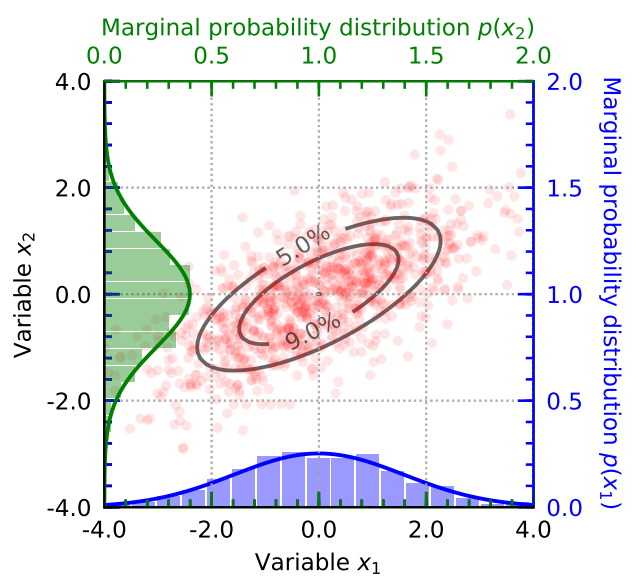
\includegraphics[scale=0.3]{02_math/02_img/multivariate_gaussian}
	}{0.49}{
		\textbf{For clarification:} $\bm{x}$ and $\bm{\mu}$ are vectors while $\bm{\Sigma}$ is a matrix.
		The probability given by $\mathcal{N}(\bm{x} \vert \bm{\mu}, \bm{\Sigma}) \in [0; 1]$ is still a scalar value!
	}
\end{frame}


% Subsection: Basic Rules of Probability
% --------------------------------------------------------------------------------------------------------
\subsection{Basic Rules of Probability}

% Basic Rules of Probability
\begin{frame}{Basic Rules of Probability}{}
	\begin{itemize}
		\item \highlight{Joint distribution:}
		\begin{equation}
			p(x, y)
		\end{equation}
		\item \highlight{Marginal distribution:}
		\begin{equation}
			p(y) = \int_x p(x, y) \diff x
		\end{equation}
		\item \highlight{Conditional distribution:}
		\begin{equation}
			p(y \vert x) = \frac{p(x, y)}{p(x)}
		\end{equation}
	\end{itemize}
\end{frame}


% Basic Rules of Probability (Ctd.)
\begin{frame}{Basic Rules of Probability (Ctd.)}{}
	\begin{itemize}
		\item \highlight{Probabilistic independence:}
		\begin{equation}
			p(x, y) = p(x) p(y)
		\end{equation}
		\item \highlight{Chain rule of probabilities:}
		\begin{align}
			\nonumber
			p(x_1, \dots, x_n)
				&= p(x_1 \vert x_2, \dots, x_n) p(x_2, \dots, x_n) \\
				&= p(x_1 \vert x_2, \dots, x_n) p(x_2 \vert x_3, \dots, x_n) \dots p(x_{n-1} \vert x_n) p(x_n) 
		\end{align}
		\item \highlight{Bayes' rule:}
		\begin{equation}
			p(y \vert x) = \frac{p(x \vert y) p(y)}{p(x)}
		\end{equation}
	\end{itemize}
\end{frame}


% Subsection: Expectation and Variance
% --------------------------------------------------------------------------------------------------------
\subsection{Expectation and Variance}

% Expectation
\begin{frame}{Expectation}{}
	\begin{alignat}{2}
		\mathbb{E}_{x \sim p(x)}\{ f(x) \} = \mathbb{E}_x\{ f \} = \mathbb{E}\{ f \}
			&= \sum_x p(x) f(x)		&&\qquad\text{\highlight{discrete case}} \\
			&= \int_x p(x) f(x) \diff x	&&\qquad\text{\highlight{continuous case}}
	\end{alignat}
	\textbf{Approximate expectation:}
	\begin{equation}
		\mathbb{E}\{ f \} = \int_x p(x) f(x) \diff x \approx \frac{1}{n} \sum_{i=1}^n f(x_i)
	\end{equation}
\end{frame}


% Expectation (Ctd.)
\begin{frame}{Expectation (Ctd.)}{}
	\begin{itemize}
		\item Some rules of expectations:
		\begin{itemize}
			\item $\mathbb{E}\{ a \bm{x} \} = a \mathbb{E}\{ \bm{x} \}$
			\item $\mathbb{E}\{ \bm{x} + \bm{y} \} = \mathbb{E}\{ \bm{x} \} + \mathbb{E}\{ \bm{y} \}$
			\item $\mathbb{E}\{ \bm{x} \bm{y} \} = \mathbb{E}\{ \bm{x} \} \mathbb{E}\{ \bm{y} \}$ (if $\bm{x}$ and $\bm{y}$ are independent)
			\item $\mathbb{E}\{ \sum_i a_i x_i \} = \sum_i a_i \mathbb{E}\{ x_i \}$
		\end{itemize}
		\item Expectations of functions:
		\begin{itemize}
			\item $\mathbb{E}\{ g(\bm{x}) \} = \int_{\bm{x}} p(\bm{x}) g(\bm{x}) \diff \bm{x}$
			\item In general: $\mathbb{E}\{ g(\bm{x}) \} \ne g(\mathbb{E}\{ \bm{x} \})$
		\end{itemize}
	\end{itemize}
\end{frame}


% Variance and Covariance
\begin{frame}{Variance and Covariance}{}
	\begin{itemize}
		\item Covariances give a measure of correlation: {\footnotesize (how much variables change together)}
		\item Scalars:
		\begin{align}
			\nonumber
			\text{cov}\{ x, y \}
				&= \mathbb{E}_{x, y} \{ (x - \mathbb{E}_x\{ x \}) (y - \mathbb{E}_y\{ y \}) \} \\
				&= \mathbb{E}_{x, y}\{ xy \} - \mathbb{E}_x\{ x \} \mathbb{E}_y\{ y \}
		\end{align}
		\item Vector notation:
		\begin{equation}
			\text{cov}\{ \bm{x}, \bm{y} \} = \mathbb{E}_{\bm{x}, \bm{y}}\{ (\bm{x} - \mathbb{E}_{\bm{x}}\{ \bm{x} \})
				(\bm{y} - \mathbb{E}_{\bm{y}}\{ \bm{y} \})^{\intercal} \}
		\end{equation}
	\end{itemize}
\end{frame}


% Subsection: Kullback-Leibler Divergence
% --------------------------------------------------------------------------------------------------------
\subsection{Kullback-Leibler Divergence}

% Kullback-Leibler Divergence
\begin{frame}{Kullback-Leibler Divergence}{}
	\begin{itemize}
		\item The \highlight{Kullback-Leibler (KL) divergence} is a similarity measure between two distributions $p$ and $q$:
		\begin{equation}
			\text{KL}(p \Vert q) = \sum_{x} p(x) \cdot \log \frac{p(x)}{q(x)}
		\end{equation}
		\item Some properties:
		\begin{itemize}
			\item It is not a distance metric: $\text{KL}(p \Vert q) \ne \text{KL}(q \Vert p)$
			\item It is non-negative: $\text{KL}(p \Vert q) \ge 0$
			\item If $\forall x: p(x) = q(x) \Rightarrow \text{KL}(p \Vert q) = 0$
		\end{itemize}
	\end{itemize}
\end{frame}


% Section: Optimization
%______________________________________________________________________
\section{Optimization}
\makedivider{Optimization}

% Subsection: Introduction
% --------------------------------------------------------------------------------------------------------
\subsection{Introduction}

% Motivation
\begin{frame}{Motivation}{}
	\begin{itemize}
		\item In every machine learning problem, you will have:
		\begin{enumerate}
			\item An \textbf{objective function} you want to optimize
			\item \textbf{Data} you want to learn from
			\item \textbf{Parameters} which need to be learned
			\item Assumptions about the problem and the data
		\end{enumerate}
		\item We would like to have general solutions to the problem of learning
		\item Different algorithms embody different objective functions and assumptions
	\end{itemize}

	\begin{boxBlueNoFrame}
		\highlight{Every machine learning problem is an optimization problem!}
	\end{boxBlueNoFrame}
\end{frame}


% Unconstrained Optimization
\begin{frame}{Unconstrained Optimization}{}
	\vfill
	\begin{center}
		\large\textbf{You know how to do that, don't you?}
	\end{center}
	\vfill
\end{frame}


% Subsection: Cost Functions and Convexity
% --------------------------------------------------------------------------------------------------------
\subsection{Cost Functions and Convexity}

% Constrained Optimization
\begin{frame}{Constrained Optimization}{}
	\vspace*{-3mm}
	\textbf{Formalization:}
	\begin{alignat*}{2}
		\min_{\bm{\theta}} \mathcal{J}(\theta)
			&= \dots 
			&&\qquad\qquad\longleftarrow\text{cost function / objective}			\\
		\text{s.\,t. } f(\theta)
			&= 0
			&&\qquad\qquad\longleftarrow\text{equality constraints}				\\
		g(\theta)
			&\ge 0
			&&\qquad\qquad\longleftarrow\text{inequality constraints}
	\end{alignat*}

	\begin{boxBlueNoFrame}
		What should an ideal optimization problem, i.\,e. the cost function and constraints look like?
	\end{boxBlueNoFrame}
\end{frame}


% Constrained Optimization
\begin{frame}{Constrained Optimization (Ctd.)}{}
	\begin{alignat*}{2}
		\min_{\bm{\theta}} \mathcal{J}(\theta)
			&= \dots 
			&&\qquad\qquad\longleftarrow\text{convex function}			\\
		\text{s.\,t. } f(\theta)
			&= 0
			&&\qquad\qquad\longleftarrow\text{linear function}			\\
		g(\theta)
			&\ge 0
			&&\qquad\qquad\longleftarrow\text{convex set}
	\end{alignat*}
\end{frame}


% Cost Functions
\begin{frame}{Cost Functions}{}
	\floattext{3.25}{4.5}{non-convex}
	\floattext{10}{4.5}{convex}
	\vspace*{4mm}
	\begin{figure}
		\centering
		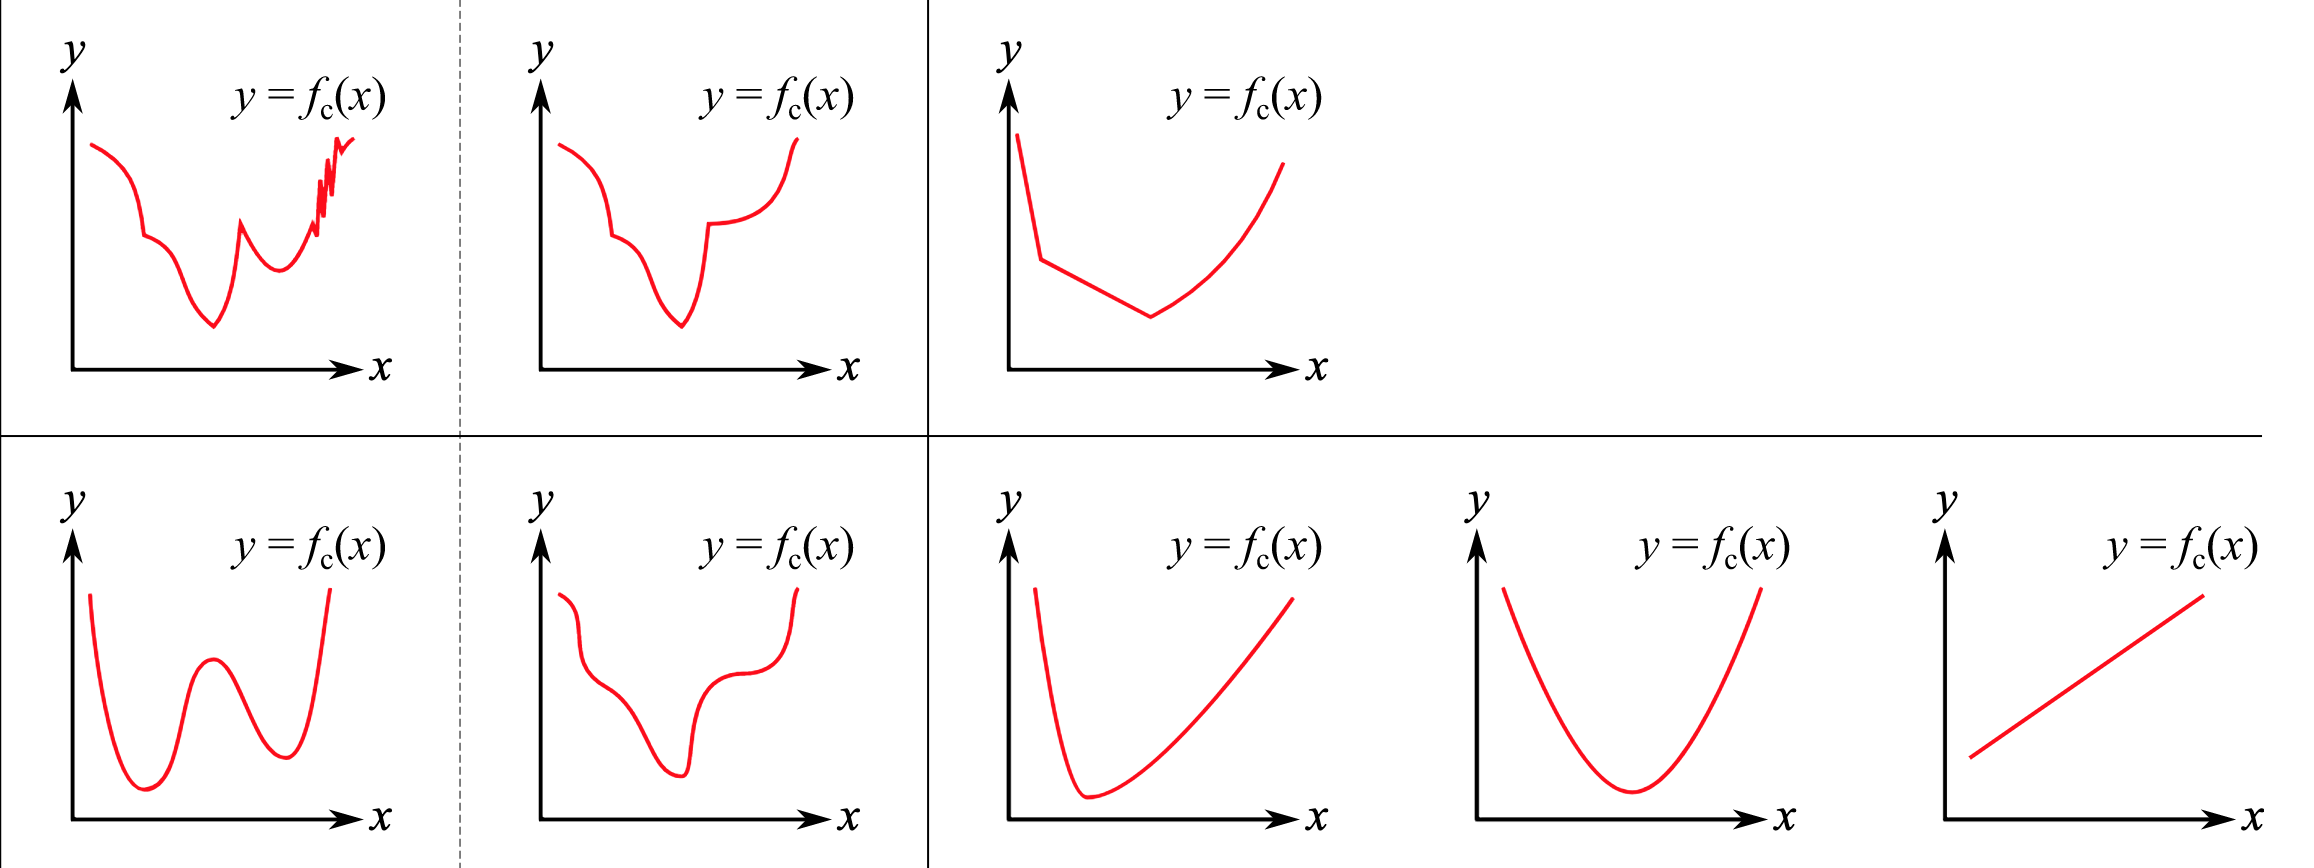
\includegraphics[width=0.9\textwidth]{02_math/02_img/cost_functions}
	\end{figure}
\end{frame}


% Convexity -- Convex Sets
\begin{frame}{Convexity -- Convex Sets}{}
	\floattext{8.75}{12}{$\bm{x}$}
	\floattext{11}{11}{$\bm{y}$}
	\floattext{2.5}{11.5}{\textbf{convex}}
	\floattext{12}{11.5}{\textbf{non-convex}}
	\begin{itemize}
		\item A set $C \subseteq \mathbb{R}^n$ is convex, if $\forall \bm{x}, \bm{y} \in C$ and $\forall \alpha \in [0,1]$
		\begin{equation}	
			\alpha \bm{x} + (1 - \alpha) \bm{y} \in C
		\end{equation}
		\item This is the equation line segment between $\bm{x}$ and $\bm{y}$
	\end{itemize}
	
	\vspace*{-3mm}
	\begin{figure}
		\center
		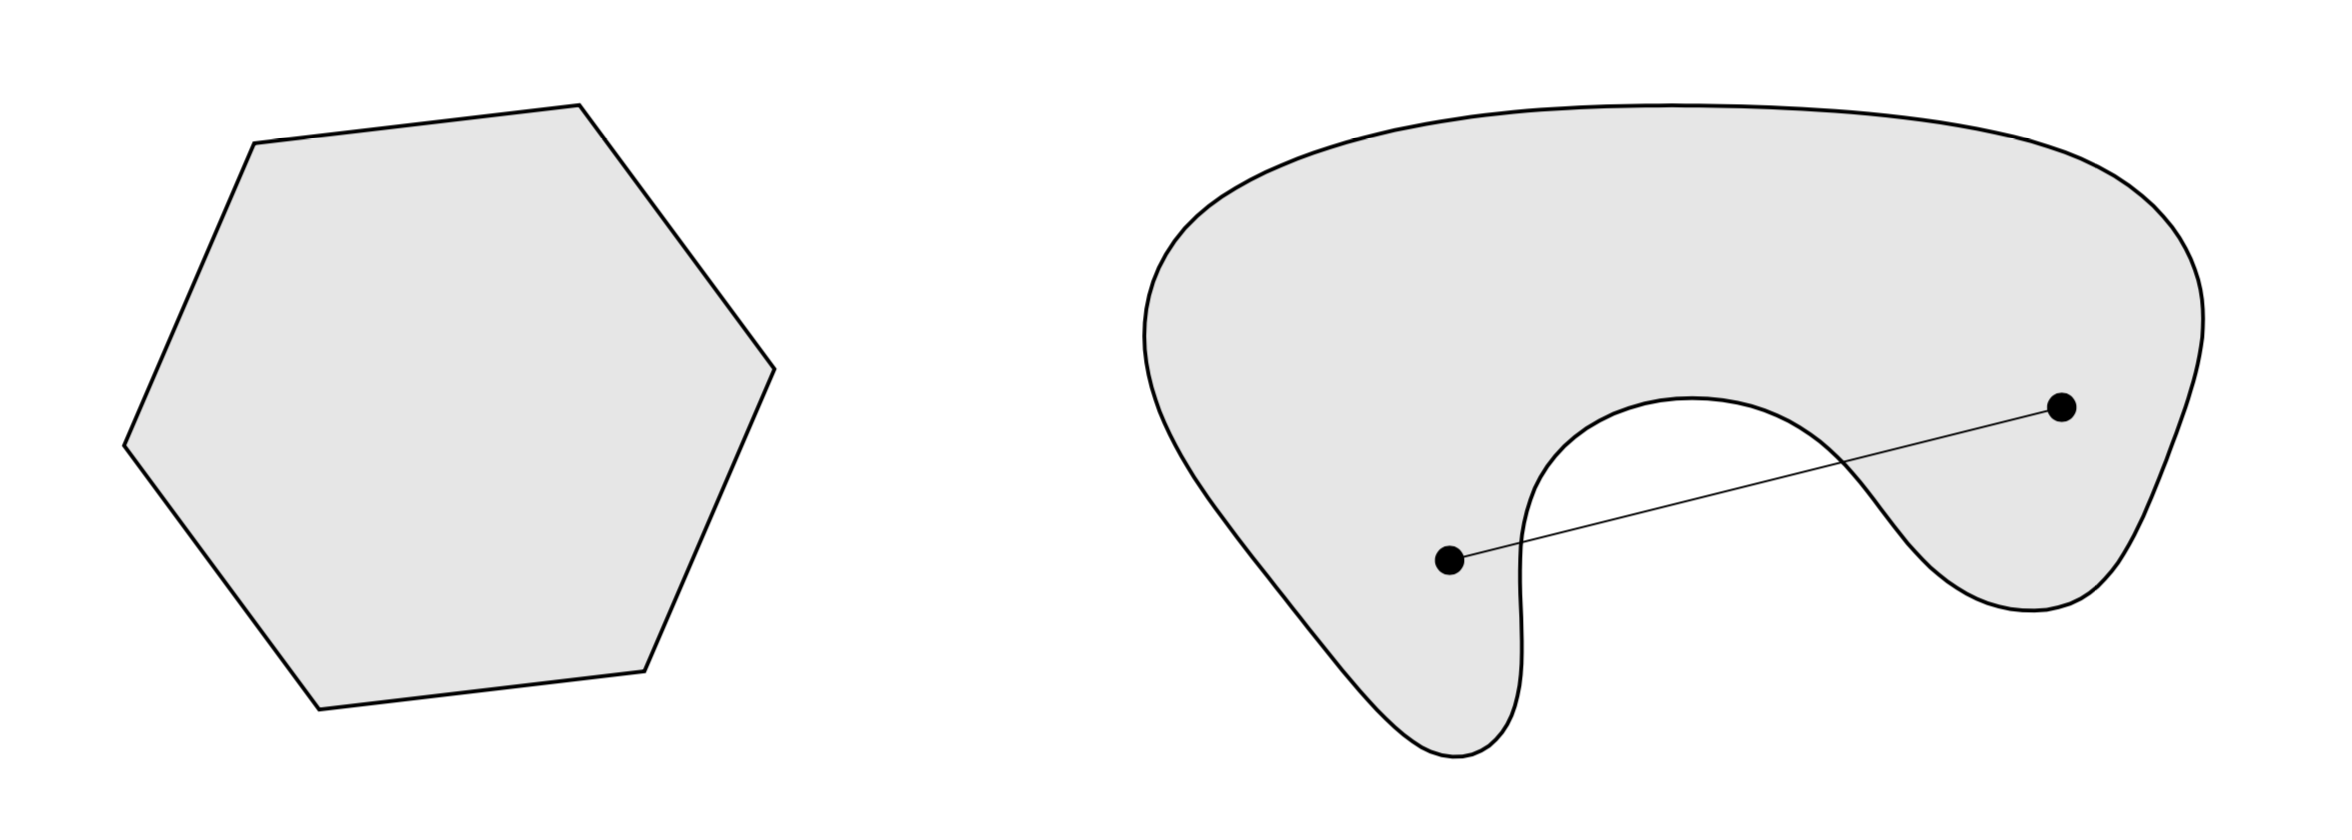
\includegraphics[scale=0.4]{02_math/02_img/convex_sets}
	\end{figure}
\end{frame}


% Convexity -- Convex Functions
\begin{frame}{Convexity -- Convex Functions}{}
	\begin{itemize}
		\item A function $f : \mathbb{R}^n \mapsto \mathbb{R}$ is convex, if $\forall \bm{x}, \bm{y} \in \text{dom}(f)$ and $\forall \alpha \in [0,1]$
		\begin{equation}
			f(\alpha \bm{x} + (1 - \alpha) \bm{y}) \le \alpha f(\bm{x}) + (1 - \alpha) f(\bm{y})
		\end{equation}
		\item Examples are linear functions $f(\bm{x}) = \bm{a}^{\intercal} \bm{x} + b$
			and quadratic functions $f(\bm{x}) = \bm{x}^{\intercal} \bm{A} \bm{x} + \bm{b}^{\intercal} \bm{x} + c$
	\end{itemize}

	\vspace*{-3mm}
	\begin{figure}
		\center
		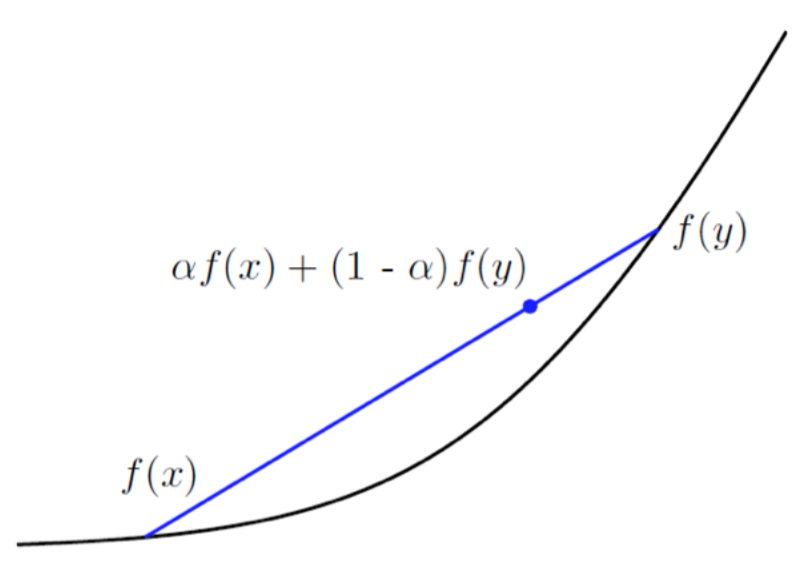
\includegraphics[scale=0.2]{02_math/02_img/convex_function}
	\end{figure}
\end{frame}


% Convexity (Ctd.)
\begin{frame}{Convexity (Ctd.)}{}
	\begin{itemize}
		\item \highlight{Why are convex cost functions so appealing?}
		\item Local solutions are global optima
		\item Efficient implementations of optimizers are available
	\end{itemize}
\end{frame}


% Subsection: Constrained Optimization and Lagrange Multipliers
% --------------------------------------------------------------------------------------------------------
\subsection{Constrained Optimization and Lagrange Multipliers}

% Constrained Optimization
\begin{frame}{Constrained Optimization}{}\important
	\begin{itemize}
		\item \textbf{How to solve this optimization problem?}
		\begin{align*}
			\min_{x, y} \mathcal{J}(x,y)
				&= 2y + x 		\\
			\intertext{subject to (s.\,t.):}
			f(x, y)
				&= y^2 +xy -1 = 0
		\end{align*}
		\item Convert the problem to an unconstrained one
		\item This is done using \highlight{Lagrange multipliers} $\alpha$
	\end{itemize}
\end{frame}


% The Concept of Lagrange Multipliers
\begin{frame}{The Concept of Lagrange Multipliers}{}\important
	\begin{boxBlueNoFrame}
		\textbf{General Lagrange function:} $\mathcal{L}(x, y, \lambda) = \mathcal{J}(x,y) + \lambda f(x,y)$
	\end{boxBlueNoFrame}

	\vspace*{3mm}
	\divideTwo{0.49}{
		\begin{align*}
			\min_{x, y} \mathcal{J}(x,y)
				&= 2y + x 		\\
			\intertext{s.\,t.:}
			f(x, y)
				&= y^2 +xy -1 = 0
		\end{align*}
	}{0.49}{
		Step \ding{182}: Differentiate w.\,r.\,t. $x$, $y$ and $\lambda$:
		\begin{alignat*}{2}
			\text{I.}\quad
				&\nabla_x \mathcal{L}
				&&= 1 + \lambda y				\\[2mm]
			\text{II.}\quad
				&\nabla_y \mathcal{L}
				&&= 2 + 2\lambda y + \lambda x 		\\[2mm]
			\text{III.} \quad
				&\nabla_{\lambda} \mathcal{L}
				&&= y^2 + xy - 1
		\end{alignat*}
	}
\end{frame}


% The Concept of Lagrange Multipliers (Ctd.)
\begin{frame}{The Concept of Lagrange Multipliers (Ctd.)}{}\important
	\divideTwo{0.49}{
		Step \ding{183}: Set equations to zero:
		\begin{alignat*}{2}
			\text{I.}	&\quad 1 + \lambda y 				&&\overset{!}{=} 0 	\\[2mm]
			\text{II.}	&\quad 2 + 2\lambda y + \lambda x 	&&\overset{!}{=} 0 	\\[2mm]
			\text{III.}	&\quad y^2 + xy - 1				&&\overset{!}{=} 0
		\end{alignat*}
	}{0.49}{
		Step \ding{184}: Substitute:
		\begin{alignat*}{2}
			\text{I.}					&\quad \lambda 		&&= -\frac{1}{y} 	\\[2mm]
			\text{I.} \rightarrow \text{II.}  	&\quad x			&&= 0			\\[2mm]
			\text{II.} \rightarrow \text{III.}	&\quad y 			&&= \pm 1
		\end{alignat*}
	}
\end{frame}


% Subsection: Numerical Optimization
% --------------------------------------------------------------------------------------------------------
\subsection{Numerical Optimization}

% Numerical Optimization
\begin{frame}{Numerical Optimization}{}\important
	\begin{itemize}
		\item Different numerical optimization algorithms exist for optimizing a function numerically on a computer if we can't solve it analytically
		\item \highlight{Gradient descent:} Incrementally update an estimate of the parameters:
		\begin{equation}
			\bm{\theta}_{new} \longleftarrow \bm{\theta}_{old} + \alpha \delta \bm{\theta}
		\end{equation}
		\item After each update: $\mathcal{J}(\bm{\theta}_{new}) < \mathcal{J}(\bm{\theta}_{old})$
		\item The algorithms differ in the number of iterations required, the computational cost, the convergence guarantees,
			the robustness with noisy cost functions and their memory usage
	\end{itemize}
\end{frame}

% Numerical Optimization Algorithms
\begin{frame}{Numerical Optimization Algorithms}{}
	\begin{itemize}
		\item \textbf{Gradient-based methods:}
		\begin{itemize}
			\item \highlight{Gradient descent} (with constant, variable step size $\alpha$)
			\item \highlight{(L-)BFGS} (Broyden-Fletcher-Goldfarb-Shanno)
			\item \highlight{Conjugate gradient descent}
		\end{itemize}
		\item \textbf{Non-gradient based methods:}
		\begin{itemize}
			\item \highlight{Genetic algorithms}
			\item \highlight{Non-Linear simplex}
			\item \highlight{Nelder-Mead}
		\end{itemize}
	\end{itemize}
	
	\begin{boxBlueNoFrame}
		\highlight{Numerical techniques may not find the global optimum!}
	\end{boxBlueNoFrame}
\end{frame}


% Gradient Descent
\begin{frame}{Gradient Descent}{}
	\begin{itemize}
		\item Most basic algorithm (and most commonly used)
		\item Go into the direction of the \textbf{steepest descent}
		\item The gradient points in the direction of the maximum ($\rightarrow$ subtract gradient)
		\begin{equation}
			\bm{\theta}^{(new)} \longleftarrow \bm{\theta}^{(old)} -
				\alpha \nabla_{\bm{\theta}} \mathcal{J}(\bm{\theta}^{(old)})
		\end{equation}
		\item The parameter updates tend to 'zig-zag' down the valley (see next slide)
		\item Gradient descent is a \highlight{1st-order method}
	\end{itemize}
\end{frame}


% Gradient Descent (Ctd.)
\begin{frame}{Gradient Descent (Ctd.)}{}
	\begin{figure}
		\centering
		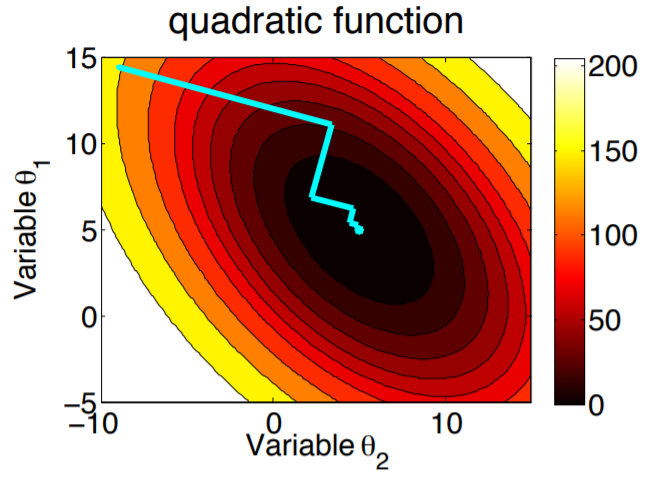
\includegraphics[scale=0.45]{02_math/02_img/gradient_descent}
	\end{figure}
\end{frame}


% Initialization
\begin{frame}{Initialization}{}
	Initialization also matters...
	\begin{figure}
		\centering
		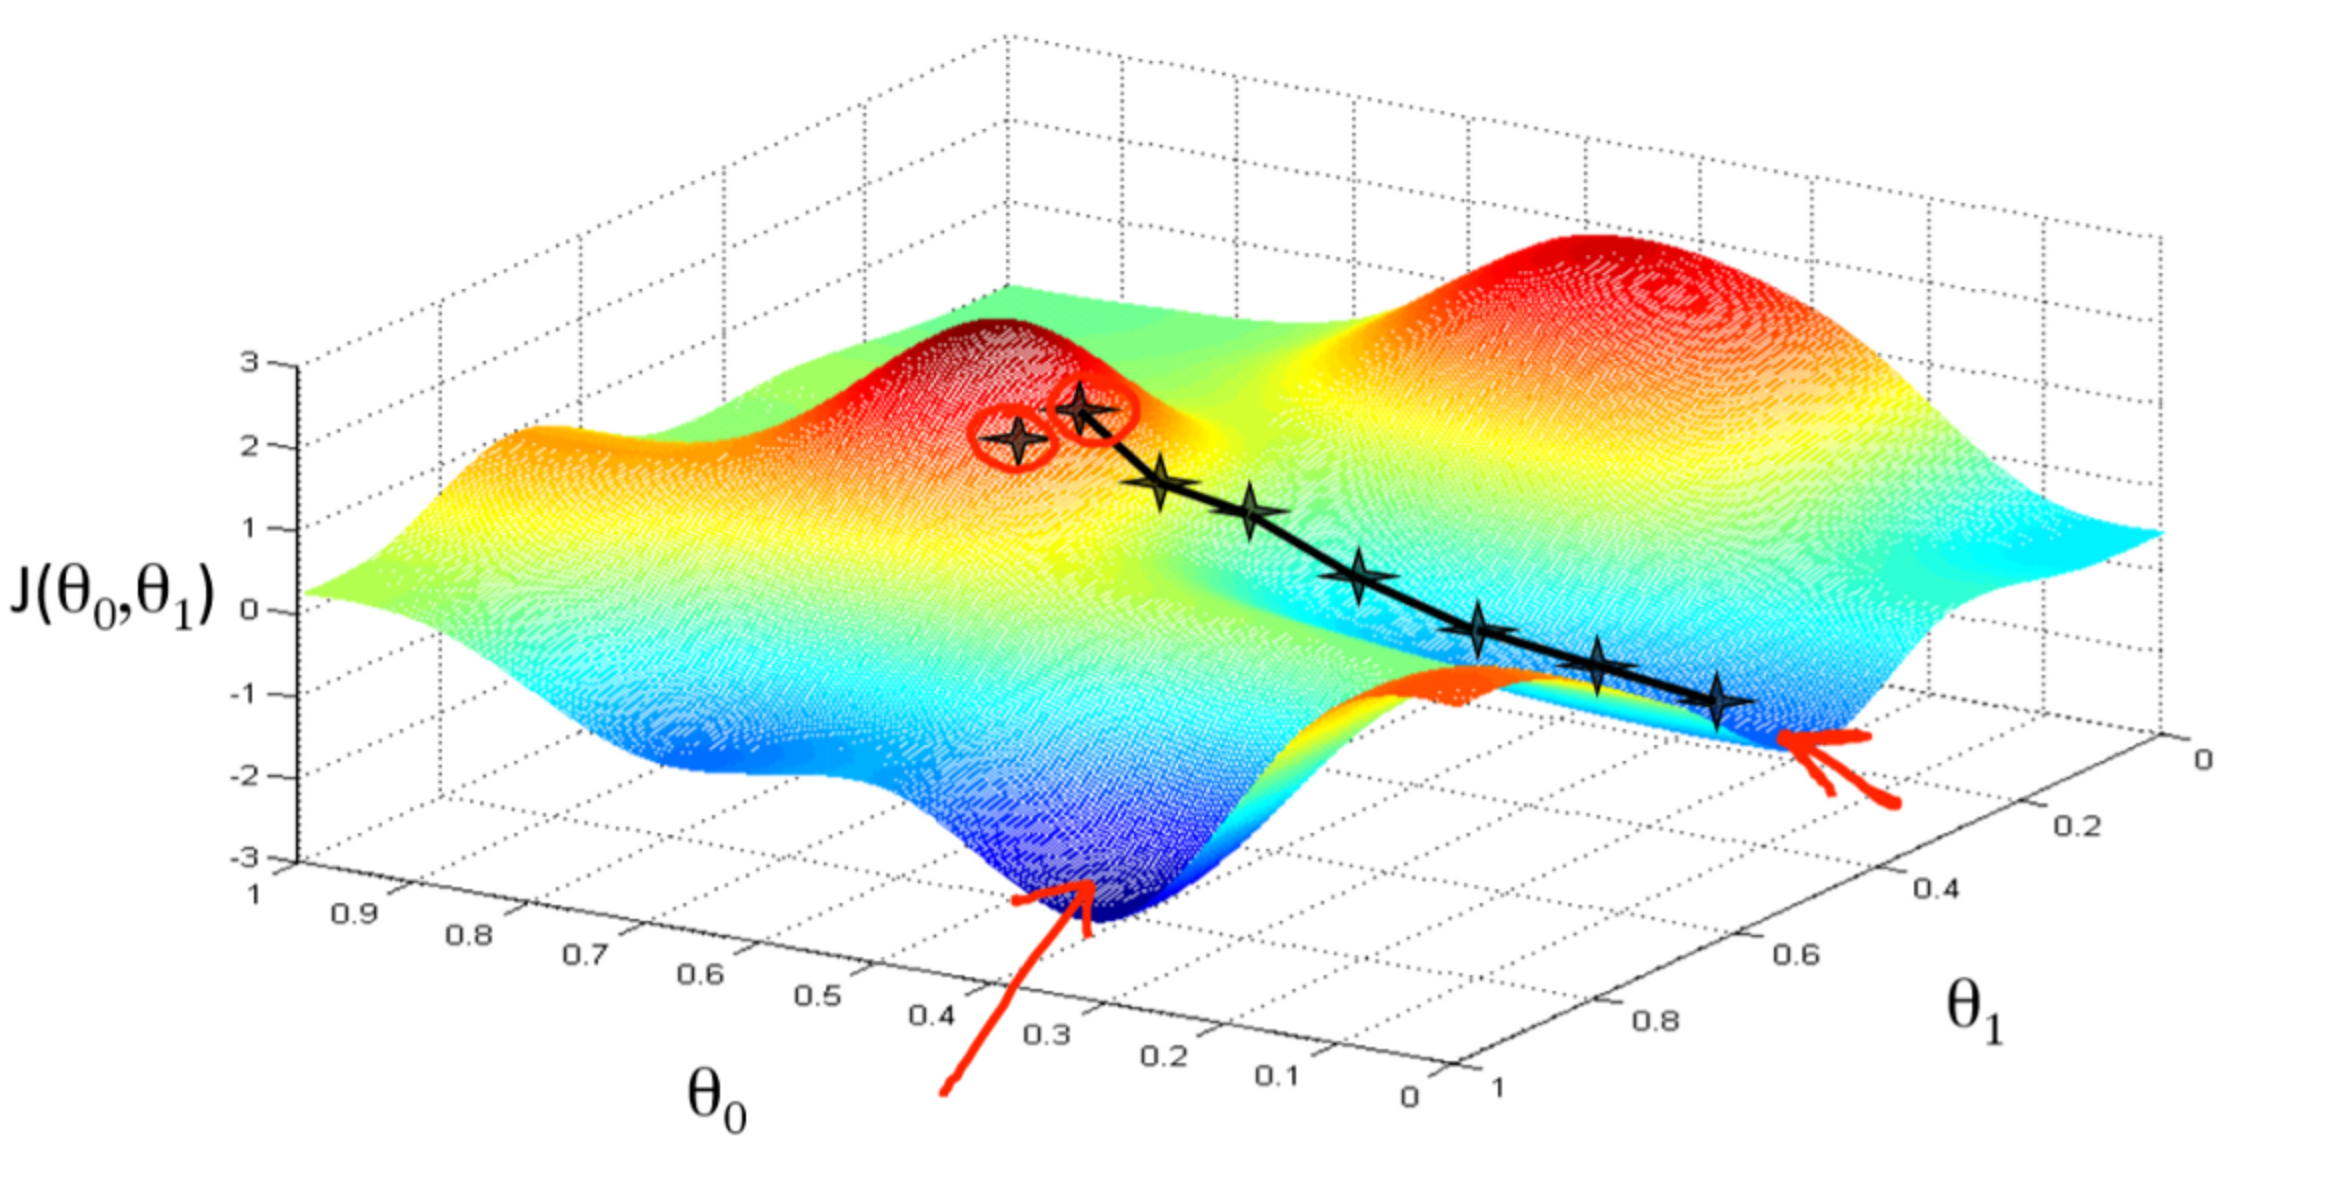
\includegraphics[width=0.75\textwidth]{02_math/02_img/gradientascent}
	\end{figure}
\end{frame}


% Newton's Method
\begin{frame}{Newton's Method}{}\optional
	\floattext{7.75}{7.5}{\footnotesize\highlight{Taylor series expansion}}
	\begin{itemize}
		\item We want to solve: {\footnotesize ($\bm{H}$ is the \highlight{Hessian}, $\bm{g}$ the \highlight{Jacobian})}
		\begin{equation}
			\delta \bm{\theta} = \argmin_{\delta \bm{\theta}}
				\left[ c + \bm{g}^{\intercal} \delta \bm{\theta} + \frac{1}{2} \delta \bm{\theta}^{\intercal} \bm{H} \delta \bm{\theta} \right]
		\end{equation}
		\item We have to differentiate and set to zero:
		\begin{equation}
			\nabla_{\delta \bm{\theta}} \left[ c + \bm{g}^{\intercal} \delta \bm{\theta} +
				\frac{1}{2} \delta \bm{\theta}^{\intercal} \bm{H} \delta \bm{\theta} \right]
				= \bm{g} + \bm{H} \delta \bm{\theta} \overset{!}{=} \bm{0}
		\end{equation}
		\item Which yields the solution:
		\begin{equation}
			\delta \bm{\theta} = -\bm{H}^{-1} \bm{g}
		\end{equation}
	\end{itemize}
\end{frame}


% Newton's Method (Ctd.)
\begin{frame}{Newton's Method (Ctd.)}{}\optional
	\begin{figure}
		\centering
		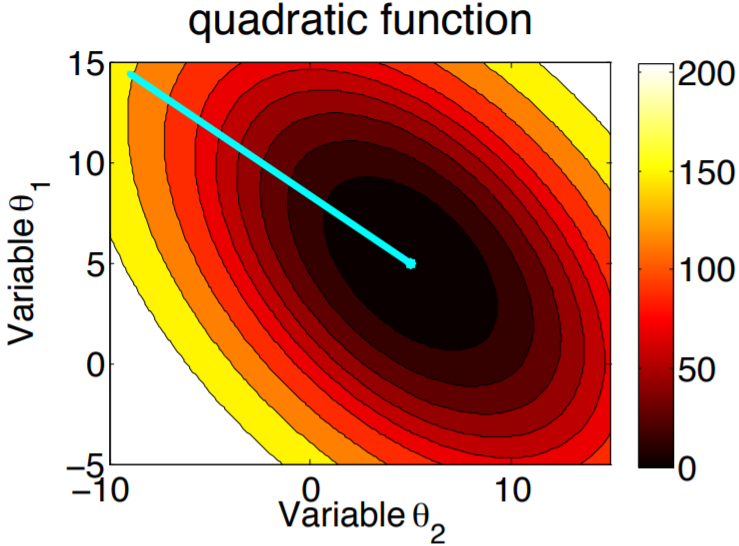
\includegraphics[scale=0.4]{02_math/02_img/newton}
	\end{figure}
\end{frame}


% Want to learn more about Optimization?
\begin{frame}{Want to learn more about Optimization?}{}
	\begin{itemize}
		\item Deep Learning book chapters 4.3, 4.4 and 8 \\
			(\href{https://www.deeplearningbook.org/contents/numerical.html}{Link chapters 4.3, 4.4},
			\href{https://www.deeplearningbook.org/contents/optimization.html}{Link chapter 8}) are highly recommended
		\item Boyd \& Vandenberghe, Convex Optimization (\href{http://web.stanford.edu/~boyd/cvxbook/bv_cvxbook.pdf}{Link})
		\item Stanford convex optimization course (\href{https://web.stanford.edu/class/ee364a/lectures.html}{Link})
		\item MOOC on constrained optimization (\href{https://www.khanacademy.org/math/multivariable-calculus/applications-of-multivariable-derivatives/lagrange-multipliers-and-constrained-optimization/v/constrained-optimization-introduction}{Link})
	\end{itemize}
\end{frame}


% Section: Wrap-Up
%______________________________________________________________________
\section{Wrap-Up}
\makedivider{Wrap-Up}

% Subsection: Summary
% --------------------------------------------------------------------------------------------------------
\subsection{Summary}

% Summary
\begin{frame}{Summary}{}
	\begin{itemize}
		\item
	\end{itemize}
\end{frame}


% Subsection: Self-Test Questions
% --------------------------------------------------------------------------------------------------------
\subsection{Self-Test Questions}

% Self-Test Questions
\begin{frame}{Self-Test Questions}{}\important
	\begin{enumerate}
		\item 
	\end{enumerate}
\end{frame}


% Subsection: Lecture Outlook
% --------------------------------------------------------------------------------------------------------
\subsection{Lecture Outlook}

\begin{frame}{What's next...?}{}
	\makeoverview{3}
\end{frame}


% Subsection: Recommended Literature and further Reading
% --------------------------------------------------------------------------------------------------------
\subsection{Recommended Literature and further Reading}

% Literature
%______________________________________________________________________
\begin{frame}{Recommended Literature and further Reading}{}
	\footnotesize
	\begin{thebibliography}{2}

	\end{thebibliography}
\end{frame}


% Thank you
%______________________________________________________________________
\makethanks

\end{document}